\documentclass[../../main.tex]{subfiles}

% Image numbers: 10-201 inclusive

\begin{document}

\newchapter{Design Process}{design-process}

\section{Preliminary design} \label{sec:design-process:preliminary-design}

\subsection{Operation and initial constraint analysis} \label{sec:design-process:preliminary-design:operation-and-initial-constraint-analysis}

To size the propulsion systems, initial analysis was conducted by estimating a number of design and environment parameters, using a normal distribution around each one to form a distribution of the most likely power requirement.
From this, early estimates of crucial parameters such as motor power, wingspan, and aspect ratio could be made.

The cruise speed was estimated using preliminary values of mass - 7kg, \cl - 0.8, aspect ratio - 10, and span - 1.8m.
The function is shown in Appendix \ref{appendix:calculation-process-for-initial-parameter-selection}.
This function could then be used to form a probability distribution, shown in Figure \ref{fig:cruise-distribution:velocity}, and hence the most likely value of the cruise velocity based on the estimated values.
It was found that the mean and median both have values of approximately \mps{21}, and so this was taken as the estimated cruise velocity during the initial phases of the project. 

The power requirements could then be estimated using a similar procedure, taking preliminary values for efficiency, mass, \vcruise \, (as estimated above), \cl, and \cd, again using normal distributions of unknown values (Appendix \ref{appendix:calculation-process-for-initial-parameter-selection}).
This was then be used to find the probability distribution for the power required in cruise, shown in Figure \ref{fig:cruise-distribution:power}.

\begin{figure}[H]
    \centering
    \begin{subfigure}[b]{0.49\columnwidth}
        \centering
        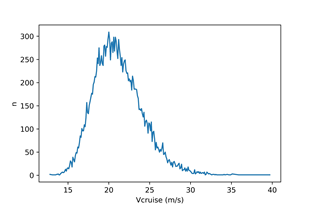
\includegraphics[width=\textwidth]{cruise-velocity-distribution}
        \caption{Velocity}
        \label{fig:cruise-distribution:velocity}
    \end{subfigure}
    \hfill
    \begin{subfigure}[b]{0.49\columnwidth}
        \centering
        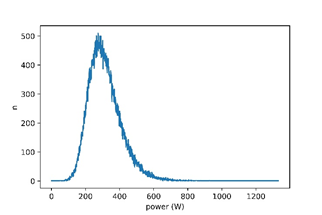
\includegraphics[width=\textwidth]{cruise-power-distribution}
        \caption{Power}
        \label{fig:cruise-distribution:power}
    \end{subfigure}

    \caption{expected distribution of selected properties during cruise.}
    \label{fig:cruise-distribution}
\end{figure}

The mean value of the power required in cruise was found to be \watts{315}, with a median of \watts{302}, giving an estimated power requirement in cruise of around \watts{310}.
There is more uncertainty in power than \vcruise\, due to the larger range of values covered within one standard deviation of the mean, but this still provided a good starting point for the project.

\subsection{Further constraint analysis} \label{sec:design-process:preliminary-design:further-constraint-analysis}

Using the refined parameters found in \S \ref{sec:design-process:preliminary-design:operation-and-initial-constraint-analysis}, design decisions made, and further analysis of the UAV, the constraint analyses were combined to show all parts of the flight profile and hence find the minimum power requirement.
This code, based in ADRpy \cite{sobester}, gave more refined estimates for the power requirement in different areas of the flight envelope, using the parameters shown in (Appendix \ref{appendix:initial-constraint-analysis}), as well as takeoff speed, which could be updated quickly and easily as design decisions were made and various operational parameters were refined.
Figure \ref{fig:constraint-analysis} shows the final plots after all research and design decisions were made.

% \importimage{full-constraint-analysis}{full constraint analysis plot with feasible region highlighted.}{Full constraint analysis}{0.85}
% \importimage{takeoff-speed-plot}{takeoff speed plot.}{Takeoff speed plot}{0.85}

\begin{figure}[H]
    \centering
    \begin{subfigure}[b]{0.85\columnwidth}
        \centering
        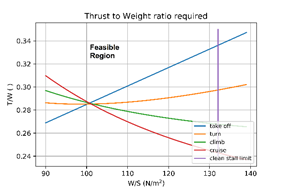
\includegraphics[width=\textwidth]{full-constraint-analysis}
        \caption{Feasible region}
        \label{fig:constraint-analysis:full}
    \end{subfigure}
    \hfill
    \begin{subfigure}[b]{0.85\columnwidth}
        \centering
        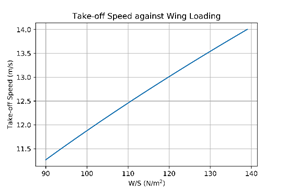
\includegraphics[width=\textwidth]{takeoff-speed-plot}
        \caption{Takeoff speed}
        \label{fig:constraint-analysis:takeoff-speed}
    \end{subfigure}

    \caption{full constraint analysis plot with the feasible region highlighted.}
    \label{fig:constraint-analysis}
\end{figure}

It can be seen that the lowest thrust to weight ratio required is around 0.29, which corresponds to a power requirement of around \watts{520}; though this is for a wing loading of only \npmsq{100}.
The final wing loading of ELMO UAV turned out to be approximately \npmsq{111}, giving a thrust to weight requirement of just over 0.3 and a corresponding power requirement of around \watts{650}, and so the final selection of motors was sufficient with a small amount of power to spare. 

\subsection{Wing} \label{sec:design-process:preliminary-design:wing}

Early in the project due to its nature, the complexity of certain components, and the limited budget, it was decided that a simple rectangular wing would be used on the UAV.
Taking the modularity onto account, a rectangular wing would reduce the number of engine housing units needed, therefore reducing the amount of design and manufacturing, and hence the cost of the project. 

The UAV had a \metres{2} span, with a fixed chord of \cm{30}, which gave an aspect ratio of 6.6.
The chord length was initially at \cm{25}, closer to the desired aspect ratio of 8.
Concerns regarding the size of flaps and ailerons were raised, however, as a significant amount of the wingspan would be lost to the motor housing units, so the chord length was increased to \cm{30} as a compromise.  

Once a wing shape had been decided, a more detailed analysis of possible aerofoil sections took place.
Initial 2D simulations were run on XFLR5 \cite{xflr-19} to narrow the choice down to five aerofoils.
The analysis was run at a Reynolds number of \stdf{1.35}{6}, calculated using standard atmospheric conditions at a cruise speed of \mps{20} and a reference length on XFLR5 of \metres{1}, tits default setting.
Although the purpose of the project was to improve the efficiency of electric aircraft by altering the position of the propulsion units, the aim was not to produce the most efficient aircraft; moreso a test craft which can be reused to run experiments at a lower cost than a wind tunnel.
Therefore, when choosing the aerofoil, the main considerations where not only $L/D$ but also stall angle, maximum \cl, and moment coefficient, amongst others. to narrow down the required analysis, aerofoils were chosen which had been recommended during research, either in papers, or on model enthusiast websites.
The analysis narrowed down to four potential aerofoils: the Clark Y, S1223, NACA6412, RG15A213, whose coordinates were taken from Airfoil Tools \cite{airfoil-tools-19}.
Figure \ref{fig:alpha-characteristics} shows the \cl, \cl$/$\cd, and \cm\, curves respectively for four suitable aerofoils. 

The Clark Y (blue line) is very common among model UAV makers because of its gentle stall angle at around \degr{12}, with a further sharper drop off at around \degr{20}.
It also has a gentle moment coefficient which makes it stable to changes in attitude during flight. 

The S1223 (black line) has an extremely high $L/D$ ratio due to its high camber; it also has a slightly higher stall angle than the Clark Y (at around \degr{14}).
It has an unfavourably large moment coefficient, however, which may make it unstable in flight.
Its high camber and narrow trailing edge may also make it difficult to implement high lift devices, as well as it not being strong enough to support a tractor propulsion set up.

The NACA6412  (green line) has a high $L/D$ ratio up to \degr{10} of incidence as well as a higher \cla\, curve, which is useful as a large part of the wing wetted area will be taken by motor housing.
It has a slightly higher moment coefficient than the Clark Y at low angle, though, as well a lower, yet gentle, stall angle of \degr{11}.

The RG15A213 (red line) has the lowest \cla\, of the five, but has a higher stall angle at \degr{15} as well as having the lowest moment coefficient.

Of the five aerofoils above, further analysis would be carried out on the Clark Y and the NACA6412 aerofoils as they provided good lift performance, strong lift to drag ratio, and a manageable moment coefficient.

\importimage{alpha-characteristics}{variation of \cl, \cl$/$\cd, and \cM\, with $\alpha$.}{Angle of attack characteristics}{0.9}

\subsection{Fuselage} \label{sec:design-process:preliminary-design:fuselage}

Given the project objectives, the design of the UAV was based around commercial aircraft, discounting any lightweight or double fuselage seen on many UAVs such as SPOTTER \cite{spotter-19}. 
Initial designs included a square, circular, and aerofoil-shaped fuselage.

\importtable{| >{\raggedright\arraybackslash}p{0.12\columnwidth} | >{\raggedright\arraybackslash}p{0.36\columnwidth} | >{\raggedright\arraybackslash}p{0.36\columnwidth} |}{
    \hline
    \textbf{Design} & \textbf{Advantages} & \textbf{Disadvantages} \\
    \hline
    Square & Easy manufacturing and wing attachment; strong structural performance & Poor aerodynamics \\
    \hline
    Circular & Easy to manufacture & Hard to attach wing; difficult to create internal structure \\
    \hline
    Aerofoil & Aerodynamic; aesthetically pleasing & Difficult to manufacture \\
    \hline
}{tradeoffs involved in the type of fuselage design.}{fuselage-tradeoffs}

\importimage{potential-aerofoil-design}{potential aerofoil fuselage design.}{Potential aerofoil design}{0.5}

For the wind tunnel model, it was decided that a hybrid of a square fuselage and an aerofoil shaped fuselage, similar to that seen in \cite{alam}, would be beneficial.
It was thought that a side profile of a NACA0012 aerofoil would reduce drag and increase lift, whilst a square front section would make manufacturing easier.
This would give a combination of aerodynamic design and ease of manufacturing.  
The NACA0012 was chosen as a suitable aerofoil as it would provide enough height to hold all of the electronics, as well as enough room to reach inside if needed. 
The initial fuselage design was \metres{1.5} long, with a width of \mm{175} and a height (at the thickest part) equal to around \mm{180}. 

\subsection{Tail} \label{sec:design-process:preliminary-design:tail}

Note that for many of the tail and control surface mathematical design processes, details of the equations used are unnecessary for understandng; but for the interested reader can been found in the appendices. 

The tail was designed with a volume coefficient process.
First, volume coefficients were estimated from Table 9.4 in Raymer \cite{raymer-89}, and a value of 0.8 was selected for the horizontal and 0.07 for the vertical tail volume.
Next, values for tail surface aspect ratios were estimated as 5 for the horizontal tail, and 2 for the vertical tail from Table 9.1 in Raymer.
The formulae for vertical and horizontal tail volume coefficients for tailplane areas were rearranged to obtain the vertical and horizontal tail areas, where the aspect ratio selected could then be used to determine span, and then MAC of the tail surfaces.
Lastly, the taper ratio was used to determine root and tip chords of the tail surfaces.
At this stage, no setting angle was determined as the need for this had not yet been recalled. 

Next, the spars had to be sized for the wind tunnel test.
Upon advice, they were sized for $10g$ loads \cite{towell-19}.
A simple mathematical beam model was used to size the spars in the tail as well as the main structural arm.
The horizontal tail spars were modelled as having a $5g$ (\newtons{49.05}) load distributed evenly over the semi-span.
Based on values for the inner and outer diameters of the spars, length, and chosen material stiffness, the tip deflection was found.
The main structural arm was determined by modelling a $10g$ point load in line with the horizontal spars, and using inner and outer widths instead of diameters, as it was decided that this would be a square section to prevent parts rotating around it.

\subsection{Systems} \label{sec:design-process:preliminary-design:systems}

The initial design was with the first wind tunnel test in mind, and as such had no plans for functional control surfaces, electronics, or avionics.
It was hoped that the first test would finalise the basics of the fuselage, wing, and tail geometry, and highlight where changes would be required from the initial design
Subsequent models and tests could validate the performance of more complex aspects of the UAV. 

Work did begin, however, on selecting and configuring a flight controller.
The primary role of the flight controller is to convert control inputs from the pilot into control inputs that are sent directly to the servos, and is normally accomplished through a range of techniques, including PID controllers.
Two main flight controllers were investigated, the first being a Pixhawk flight controller $-$ more expensive, but potentially more useful and had been used by people at the university before $-$ and the second being a Matek F405-Wing board with iNav Flight firmware installed on it. 

While the Pixhawk could have been easier to set up, with its advertised plug-and-play functionality, it was significantly more expensive, and so it was decided that looking into the Matek controller could be worth a potentially large saving (albeit with a greater risk of purchasing the controller to find that it did not work as expected).
The Matek hardware came at about half the cost of the Pixhawk, and while the corresponding firmware was relatively immature, its open source nature meant that its functionality was expanding quickly, and it had favourable reviews from a number of online sources.
Another potential advantage of the Matek controller was that it was designed specifically with fixed wing aircraft in mind, whereas the Pixhawk was focused more towards quadcopters. 

\importimage{matek}{pin layout and documentation for the Matek flight controller.}{Flight controller layout}{0.95}  % TODO: include source (http://www.mateksys.com/?portfolio=f405-wing)

Other beneficial features of the Matek board were the built-in current sensor and inertial measurement unit (IMU) which would provide estimates of the position, and more importantly orientation, of the UAV.
There were also a number of fairly low-cost GPS and airspeed sensor units, required for the latter part of the avionics system's specification of providing autopilot functionality. 

\importimage{flight-configurator}{flight configurator software used to set up the flight controller.}{Flight configurator}{0.6}

Input to the flight controller could be achieved through a number of protocols, most notably through SBUS; this type of serial connection appeared to be the most commonly supported amongst receivers, and would allow up to sixteen channels to be passed from the receiver to the controller.
The minimum required channels would be eight: four for throttle, yaw, pitch, and roll; two for flaps (on/off); and similarly two for the autopilot toggle.
With the additional channels it would in principle be feasible to implement extra features, such as manually cutting off outboard motors in the event that one of them should fail. 

Also of interest were the UART ports (Figure \ref{fig:matek}), which is a serial communication protocol broadly compatible with a number of microcontrollers, including Arduinos.
This would be a good option for extracting the data from the current sensor and passing it to a microcontroller $-$ most likely an Arduino Nano $-$ which could then integrate the current draw over time to provide an estimate of the battery capacity used by a particular configuration.
Being able to do this onboard was appealing because the need for telemetry, which would have significantly increased the complexity of the radio system, could be removed.
All data could be logged by a relatively simple program, written in C++, to be downloaded after each flight.

Small GPS and airspeed modules were also found online which were designed specifically to be compatible with the Matek F405-Wing.

\importimage{flight-controller-computer}{flight controller plugged into a computer running the flight configurator.}{Flight controller configuration}{0.6}

\subsection{Propulsion} \label{sec:design-process:preliminary-design:propulsion}

\subsubsection{Twist-in motor attachment} \label{sec:design-process:preliminary-design:propulsion:twist-in-motor-attachment}

\begin{figure}[H]
    \centering
    \begin{subfigure}[b]{0.49\columnwidth}
        \centering
        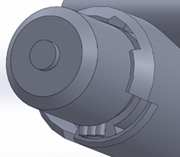
\includegraphics[width=\textwidth]{twist-in-in-place}
        \caption{Motor in-place in housing}
        \label{fig:twist-in:in-place}
    \end{subfigure}
    \hfill
    \begin{subfigure}[b]{0.49\columnwidth}
        \centering
        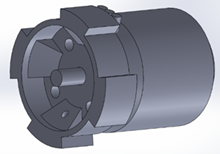
\includegraphics[width=\textwidth]{twist-in-attached}
        \caption{Bracket attached to motor}
        \label{fig:twist-in:attached}
    \end{subfigure}

    \begin{subfigure}[b]{0.49\columnwidth}
        \centering
        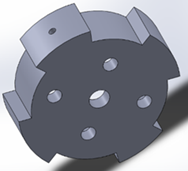
\includegraphics[width=\textwidth]{twist-in-bracket}
        \caption{Bracket}
        \label{fig:twist-in:bracket}
    \end{subfigure}
    \hfill
    \begin{subfigure}[b]{0.49\columnwidth}
        \centering
        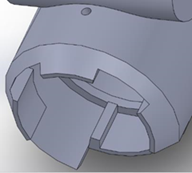
\includegraphics[width=\textwidth]{twist-in-housing}
        \caption{Housing}
        \label{fig:twist-in:housing}
    \end{subfigure}
    \caption{CAD models of the twist-in motor attachment used in the tail.}
    \label{fig:twist-in}
\end{figure}

Conceived early in the project's development, the twist-in motor attachment (Figure \ref{fig:twist-in}) was a proposed design for the attachment of the wing motors.
When the design criteria changed to include a battery and ESC in the movable propulsion unit, a new design was required.
This design, however was still used in the tail section as the battery and ESC were fixed in the fuselage for that configuration, and so only the motor moves, making this an ideal solution.

The design is intended to allow for quick and simple removal and replacement of the motor when changing configurations of the UAV in order to reduce ground time at the flying days.
This utilises a twist and fix design where four tabs on the bracket, shown in Figure \ref{fig:twist-in:bracket}, which attaches to the back of the motor as shown in Figure \ref{fig:twist-in:attached}, engage with four tabs in the housing, and the motor then rotates up to a limiting piece to align the bracket and housing (Figures \ref{fig:twist-in:housing} and \ref{fig:twist-in:in-place}).
The motor is then secured in place using a small grub screw which engages with the bracket through a clearance hole in the top of the housing, as shown in Figure \ref{fig:twist-in:housing}, providing resistance to rotation of the motor while the tabs provide the strength in the direction of the force of the motor.
The large cut-out in the housing is to allow room for the wires of the motor when it is being fitted, as they protrude from the rear part of the motor out to the side, shown in Figure \ref{fig:twist-in:in-place}.
On the final design for the tail there is a full routing designed for the wires but that was not designed here as this housing was intended for the wing before being deprecated.

\subsubsection{Sizing} \label{sec:design-process:preliminary-design:propulsion:sizing}

Initial sizing started from the constraint analysis' power requirement estimations, allowing motors to be selected.
The constraint analysis at this point suggested a power requirement of around \watts{600}, and so motors of around this power were researched from a recommended supplier Outlander, and a number of suitable cost-effective motors were found for both the fuselage and wing locations.
These were then used to find suitable ESCs, which were recommended for the motors as \amps{60} and \amps{30}, but due to this being the most common part to fail on previous projects due to overloading, a decision was made to oversize the ESCs by \pc{30} and so \amps{40} and \amps{80} ESCs were selected.
The batteries were then chosen based on the voltage and current requirements of the motors, meaning that they needed to be 4S to provide the required \volts{14.8}, and the capacity initially chosen simply on weight and cost, with the largest capacity shown being the heaviest that could be used.
The C value is used to find the maximum current output of the battery and so this was chosen to ensure a large safety margin between the maximum of the battery and the maximum of the motor, reducing any chance of the battery overheating while in use. 

The motor selection was then refined due to an increase in the power requirement prediction from the constraint analysis resulting from updates to the UAV design; this meant that the motors could be selected as the Tornado Thumper V3 3548/05 and 3530/14 for the fuselage and wing motors respectively.
This meant that the battery capacities could be checked for time of flight based on an estimated \pc{75} throttle average throughout a flight.
While this is an overestimate, it gives a useful conservative estimation of the flight time.
This showed that the smaller capacity batteries would not be enough to provide a flight time suitable for recording the needed data while having a margin in the battery to avoid a power cut-out mid-flight.

Along with finalising the battery selection, the propellers could now be researched.
This initially required the maximum propeller diameter to be found for the motors, based on the max RPM of the motor, which would give a Mach number of the propeller of around 0.7, which would maximise thrust without having large increases in power requirement due to transonic effects at the blade tip.
This was then used to refine an iterative search of the available propellers from APC, a manufacturer trusted by the university.
The advance ratio was found based on the blade diameter, RPM, and a target maximum flight speed of \mps{25}, and then a suitable propeller was found in the database that had a power draw similar to that of the maximum of the motor at the target flight speed and RPM, while providing enough thrust based on estimations of the aircraft drag.

These propellers were checked after selection at the target cruise speed of \mps{20} to ensure that the thrust would be adequate, and to find an estimation of the efficiency in order to further refine the constraint analysis.
The ideal propellers, however, could not be used due to the specific use case of the project, which requires both tractor and pusher configurations to be employed, as well as counter rotating propellers on each wing; this meant that the propeller would need to have an equivalent pusher propeller.
The selection of propellers was therefore forced into suboptimal blades, with the fuselage propeller only having one viable option of the APC 12x6E and 12x6EP propellers, and the wing having two options of the 8x6E and 7x5E.
After analysis of thrust data, the 8x6E was chosen to be used in a motor and propeller wind tunnel test to verify that this propeller would be suitable, and to verify the quoted performance data in order to ensure that the 12x6E would also be suitable. 

\section{Physical testing and validation} \label{sec:design-process:physical-testing-and-validation}

\subsection{Wind tunnel test} \label{sec:design-process:interim-design-review:wind-tunnel-test}

\subsubsection{Fuselage} \label{sec:design-process:interim-design-review:wind-tunnel-test:fuselage}

The fuselage was designed around a hollow \metres{1} long and \mm{20} square aluminium boom as its core structural element.
Around the boom was a foam and poplar plywood structure, similar to the wing. 

The driving force behind the fuselage design was the need to be able to change the setting angle of the wing between tests with ease.
As a result, the metal boom was fixed to four layers of poplar ply ribs which ran the length of the fuselage. 

To allow the wing setting angle to be changed easily, three sets of holes ran through the fuselage.
The front set of holes were a tight fit for the front spar, so it could not move.
The middle set was a guide for the rear spar to help changing the angle.
The rear set of holes were to secure the wing in place.
This section contained seven holes in total, each \degr{2} apart, meaning the wing's angle could be changed from \degr{0} up to \degr{12}. 

\importimage{fuselage-cross-section}{a cross-section of the fuselage, showing the structure and hole layouts.}{Fuselage cross-section}{0.6}

At the rear of the model, on the underside, the middle two ribs contained an attachment point for the wind tunnel.
This was extruded from the model to enable the model to be easily attached and removed from the struts. 

\importimage{laser-cut-plywood}{laser-cut plywood for the fuselage.}{Laser-cut plywood}{0.7}

\subsubsection{Wing} \label{sec:design-process:interim-design-review:wind-tunnel-test:wing}

The wing was constructed using two hollow aluminium spars as the key structural elements with the front spar at quarter chord and the rear spar at half chord, with outer diameters of \mm{15.88} and \mm{12.7}, respectively.
Each spar was \metres{2} long and ran tip to tip through the fuselage.
Surrounding the spars was blue styrofoam, cut in the university's foam cutter.
Separating the foam sections were \mm{3} thick poplar ply ribs, cut on university's laser cutter.
Each rib had a unique design and were individually designed and cut.

\importimage{flap-dfx-file}{DFX file of flap rib for the Clark Y aerofoil section, later used for laser cutting.}{Flap DFX file}{0.6}

There were six ribs used in each wing half, in locations that would roughly replicate where the motor housing units would be on the final model.
Therefore, the ribs were located either side of the flap and \mm{130} outboard.
The next rib, located \mm{101} outboard, was the rib used to connect the model to the wind tunnel.
Therefore, it was made from \mm{6} birch ply as this provided sufficient strength for an integral component.
The two final ribs were located at the wing tip and \mm{50} inboard.

\importimage{underside-of-wing}{the underside of the wing, showing attachment and flap adjustment methods.}{Underside of wing}{0.6}

The thicker birch ply rib, located \mm{700} outboard of the centre of the aircraft, contained an extrusion with a hole for an M6 bolt to allow easy attachment and removal to the wind tunnel mounts.
Its location along the wing was dictated by the wind tunnel mounts. 

\importimage{clamp-wt}{wingtip clamp CAD model.}{Clamp wingtip}{0.6}

The foam and ribs for each side of each wing were bonded together using epoxy resin but were not bonded to the spars themselves, allowing the wing sections to be removed from the spars during the wind tunnel test. 
The wings were secured to each spar by using 3D printed clamps (Figure \ref{fig:clamp-wt}) imbedded in the wing's strucure.
These were attached to the wings' ribs using epoxy based bonding agent.
Two M3 bolts allowed to tighten the clamps onto the spars, thus securing the wing assembly.

\importimage{internal-spar-structure}{Wing section showing the internal spar structure.}{Internal spar structure}{0.6}

\subsubsection{Control surfaces} \label{sec:design-process:interim-design-review:wind-tunnel-test:control-surfaces}

The main purpose of the wind tunnel model was to cement top level parameters such as aerofoil section, setting angle, chord length, and wingspan.
As a result, the wind tunnel was unpowered, and ailerons were not included in the model.
It was, however, important to test the effect of a flap on each wing and which aerofoil would be more amenable to the addition of a flap. 

Initial research suggested that, for a typical low-speed UAV, ailerons take up approximately \pc{40} of the semi-span, in this case \mm{400} \cite{sadraey-13}.
This left the remaining \pc{60} for flaps.
The design at the time, however, called for the motor housing units to have width of approximately \mm{110}.
There would be two located on each half of the wing, and a tip mounted motor, whose depth had not yet been determined.
The flaps were therefore set to a width of \mm{380}, which would act as a worst case scenario approach to the design, and would provide each wing section with a strong test.

The flaps were designed to be changed manually whilst the model was still attached to the wind tunnel.
The guides either side of the flaps had M2 holes every \degr{5} up to \degr{35}.
As the flap angle was altered, two M2 bolts would secure the flap in place. 

\importimage{flap-mechanism}{close up of the flap mechanism.}{Flap mechanism}{0.6}

\subsubsection{Tail} \label{sec:design-process:interim-design-review:wind-tunnel-test:tail}

With the mathematical modelling complete, a 3D model of the tail surfaces could be created as reference for building.
This was done by defining the sketch planes upon which the roots and tip chord aerodynamic profiles would be created, importing curves of the aerofoil from coordinate files, and parametrising them (by chord length and angle of attack) so that they could be manipulated.
Lofted bases were created between the profiles, then additional details such as cut-outs for spars were added.
This was repeated for all three control surfaces, and then simple models of the tail spars and main structural arm were created and added to the overall assembly. 
The initial plan was to use the foam cutter to create the tail profiles, however, this proved to be infeasible as the cut-outs for the spars in a thin aerofoil profile (NACA0012) left very little foam in the wall which resulted in the foam melting at the tip where the cutter had to slow down.  

There was not enough time to redesign the tail because of the upcoming test, so it was decided to laser cut wooden profiles at equally spaced intervals along the tail surfaces and wrap Solarfilm around them.
Geometry was created in CAD using repeated \mm{3} profiles intersecting the foam geometry, and then non-intersecting geometry was deleted to leave the laser cut profiles, which were quickly exported and cut.
Each profile was mounted and bonded to the spar.
Once the glue had cured, Solarfilm was wrapped around the profiles, with the leading and trailing edges stiffened with card.
While this was messy, it was effective; it was resolved to refine the model for the next iteration of the design.  

The tail was mounted on the model using a friction fit with the spars running through the fuselage and main structural arm.
Holes were drilled through these that were intentionally half a millimetre short of the spacing required.
One horizontal tail surface was glued to one spar, and the other to the second, so they would slot together neatly in the model.
The vertical tail surface contained both spars, and simply slotted in all at once. 

\importimage{wind-tunnel-model}{final wind tunnel model.}{Wind tunnel model}{0.8}

\subsubsection{Test plan} \label{sec:design-process:interim-design-review:wind-tunnel-test:test-plan}

The wind tunnel test had a few objectives.
The first was to validate the designs produced so far, ensuring that lifting surfaces could produce sufficient lift and were able to withstand the predicted structural loads.
Assuming these conditions were met, a combination of aerofoil, wing-body angle, and flap-wing angle needed to be found which optimised the objective function (discussed later in more detail).
Data collected during this optimisation would also be used afterwards to refine the design further $-$ by estimating the change to lift or drag that would result from changing the size of the flaps $-$ and to validate the accuracy of CFD simulations. 

Five variables were controllable within the wind tunnel: aerofoil, the angle between the wing and the fuselage (wing-body angle), the angle between the flaps at maximum deflection and the wing (flap-wing angle), angle of attack, and airspeed.
The experiment space created by all of these variables is much larger than would have been feasible to explore fully within one wind tunnel session, and so the testing was split into two phases $-$ cruise and takeoff $-$ and some simplifications were made to enable a subset of the experiment space to be explored while still yielding near-optimal results.

During cruise, some of the variables could be fixed.
Angle of attack was to be set to \degr{0}, cruise speed was to be fixed at \mps{20}, and flaps were not to be kept retracted.
The experiment space then consisted of the two aerofoil options and a number of wing-body angle settings for each one, and was further reduced by assuming that an increase in wing-body angle would always correspond to an increase in drag, and would cause an increase in lift as long as the wing had not stalled.
The objective function for the cruise phase of testing could then be defined as the combination of aerofoil and wing-body angle which minimise drag while producing at least \newtons{70} of lift, and then the wing-body angle could be gradually increased for each aerofoil until the lift exceeded \newtons{70}, at which point the testing for that aerofoil would be terminated. 

After the cruise phase of testing had been completed, the optimal aerofoil section and wing-body angle were to be held constant for the takeoff phase of testing.
If a takeoff speed of \mps{12} is assumed, the experiment could alter the flap-wing angle and angle of attack (to account for bumps or irregularities in the runway) to find a flap-wing angle which maximises $L/D$ while still providing sufficient lift for takeoff at the minimum takeoff angle and not stalling at the maximum takeoff angle.
Reasonable maximum and minimum takeoff angles were determined from assumptions about the size and length of the landing gear, and the amplitude of bumps on the takeoff surface.
Varying the angle of attack between these two bounds would not not cost an excessive amount of time as, unlike the flap-wing angle, that parameter could be varied without the wind tunnel being turned off. 

This procedure was written up into a testing plan, whose conditions enabled the design space to be suitably explored without taking up too much time.
Care was taken to ensure that the plan was objective and covered all edge cases (barring extreme edge cases, such as no configurations producing the required amount of lift or structural failure, which would require a more thorough redesign of the aircraft) so that the results did not need to be discussed during the course of testing.
As much time as possible could then be spent changing the model between the required configurations; estimates of how long would be needed to vary each parameter were also made.

Provisions were also made for gathering data to analyse the stability of the model if there was any time left over at the end of these two testing phases.
With the optimal aerofoil section and wing-body angle according to the objective functions described above, and flaps fully retracted, forces and moments on the model were to be measured for a range of airspeeds and angles of attack.
Since both of these parameters were variable without turning off the wind tunnel, a relatively large amount of data could be collected fairly quickly.
Once a suitable amount of data were collected, similar sweeps of the parameter space with the optimal configuration would be made with the tail taken off.

\subsubsection{Results and analysis} \label{sec:design-process:interim-design-review:wind-tunnel-test:results-and-analysis}

The results from the wind tunnel test required considerable post-processing before analysis could be carried out, but once this was complete the graphs could be made and the results easily analysed.
There was a significant problem when the correction for the drag of the mounting structure, used to hold the model in the wind tunnel, was implemented because it caused some of the drag results to be negative.
The drag data were therefore unreliable, but the trends seen in the results could still be useful.
The drag data will now rely on CFD and additional wind tunnel tests for clarification.

Figure \ref{fig:wind-tunnel-results:wing-setting-angle} shows the results from the initial test carried out, where the setting angle of the two wings were found by increasing the angle of the wing against the fuselage until the lift exceeded the target weight of \newtons{70} at the target cruise speed of \mps{20}.
This graph shows that the NACA6412 exceeded this lift at \degr{1}, and so was set at \degr{2} for the rest of the test to give a margin as the final wing is expected to produce slightly less lift due to the attachment of the propulsion units.
The Clark Y exceeded the required lift at around \degr{3} and so was set at \degr{4} for the same reason.  The differences in lift are due to the higher camber on the NACA aerofoil.

Figures \ref{fig:wind-tunnel-results:lift-comparison} and \ref{fig:wind-tunnel-results:drag-comparison} show the comparison between the NACA6412 and Clark Y wings through a full sweep of angle of attack.
At this point the wings were set at their optimal angles, and so the whole model was moved through the range of angles of attack to give the data.
It can be seen that the two wings produce very similar \cl\, values; while this is expected since the wings are set at their optimal angles, the Clark Y aerofoil stalls before the NACA6412, thus giving a lower maximum lift.
This is one of the reasons the NACA6412 was chosen as the aerofoil for the final UAV instead of the Clark Y.
It can also be seen that the Clark Y has a higher \cd\, at all angles of attack, and so is less efficient than the NACA6412.

Figures \ref{fig:wind-tunnel-results:naca-lift-coefficient} through \ref{fig:wind-tunnel-results:cl-against-cd} show the plots for the wind tunnel model equipped with the NACA6412 at a range of airspeeds, showing the performance throughout the target flight envelope of the UAV.
Figure \ref{fig:wind-tunnel-results:naca-lift-coefficient} shows that the \cl\, remains almost constant as the airspeed changes and that, as expected, there are no compressibility effects as these speeds. The slight differences are due to changes in the boundary layer development at the different Reynolds numbers
Figure \ref{fig:wind-tunnel-results:naca-drag-coefficient} shows that the \cd\, reduces with the increase in airspeed, which is due to the variation of $C_\mathrm{D,0}$ and $C_\mathrm{D,i}$ with airspeed.
Figure \ref{fig:wind-tunnel-results:cl-against-cd} shows that the highest aerodynamic efficiency is therefore found at the highest tested speed of \mps{22}, and although this speed is above the targeted cruise speed of the UAV, one can conclude that to maximise range the UAV should be flown above the intended cruise speed. 

Figures \ref{fig:wind-tunnel-results:flap-drag-comparison} and \ref{fig:wind-tunnel-results:flap-lift-comparison} show the results of the flap test that was performed with the NACA6412 wing.
Figure \ref{fig:wind-tunnel-results:flap-drag-comparison} shows the increase in \cd\, that comes with each increment of the flap angle, while Figure \ref{fig:wind-tunnel-results:flap-lift-comparison} shows that the \cl\, increases significantly with the flaps activated but that the variation of the flap angle has little to no effect on the increase in \cl.
This suggests that the flaps are stalling at \degr{30}, and so the flap angle to be used in the final model was chosen to be \degr{30}.
Figure \ref{fig:wind-tunnel-results:30-degree-flap-lift} shows that the lift increase was not enough to provide the required lift at the target takeoff and landing speed of \mps{12}, with the maximum lift produced being just under \newtons{60} at \degr{10}.
The wing had not stalled at this point and so there was the possibility that the wing could produce more lift at a higher angle of attack, though this could not be tested as \degr{10} was the highest wing-body angle that could be reached.
Even so, it became clear that the design of the flaps needed to be modified to improve their effectiveness, and also that the area of the wing used for the flaps should be increased in order to maximise their effectiveness. 

The wind tunnel test also provided data for the pitching moment about the aerodynamic centre of the wing, as shown in Figure \ref{fig:wind-tunnel-results:moment-coefficients}, which gives an insight into the aerodynamic stability of the model and the pitching moment developed by the wing.
The data show that the coefficient of pitching moment is independent of airspeed and is negative at \degr{0} angle of attack, which is less than ideal since it implies that the aircraft would be trimmed at \degr{-3} angle of attack corresponding to higher than the intended cruise speed, thus requiring the pilot to trim the model or use constant elevator in order to fly level at any cruise speed or slower.
The negative gradient of the line on the plot is good, however, as it implies that the aircraft is aerodynamically statically stable in pitch, so any pitching up of the aircraft would produce an increase in the pitching down moment and the aircraft would automatically stabilise.
Furthermore, with an adjustment to the tailplane, the magnitude of the pitching moment could be made zero at \degr{0} angle of attack by producing a counteracting moment with an angled tailplane, meaning that the pilot would not need to trim the aircraft to the same extent. 

\newcommand{\multiimagewidth}{0.4}

\begin{figure}[H]
    \centering
    \begin{subfigure}[b]{\multiimagewidth\columnwidth}
        \centering
        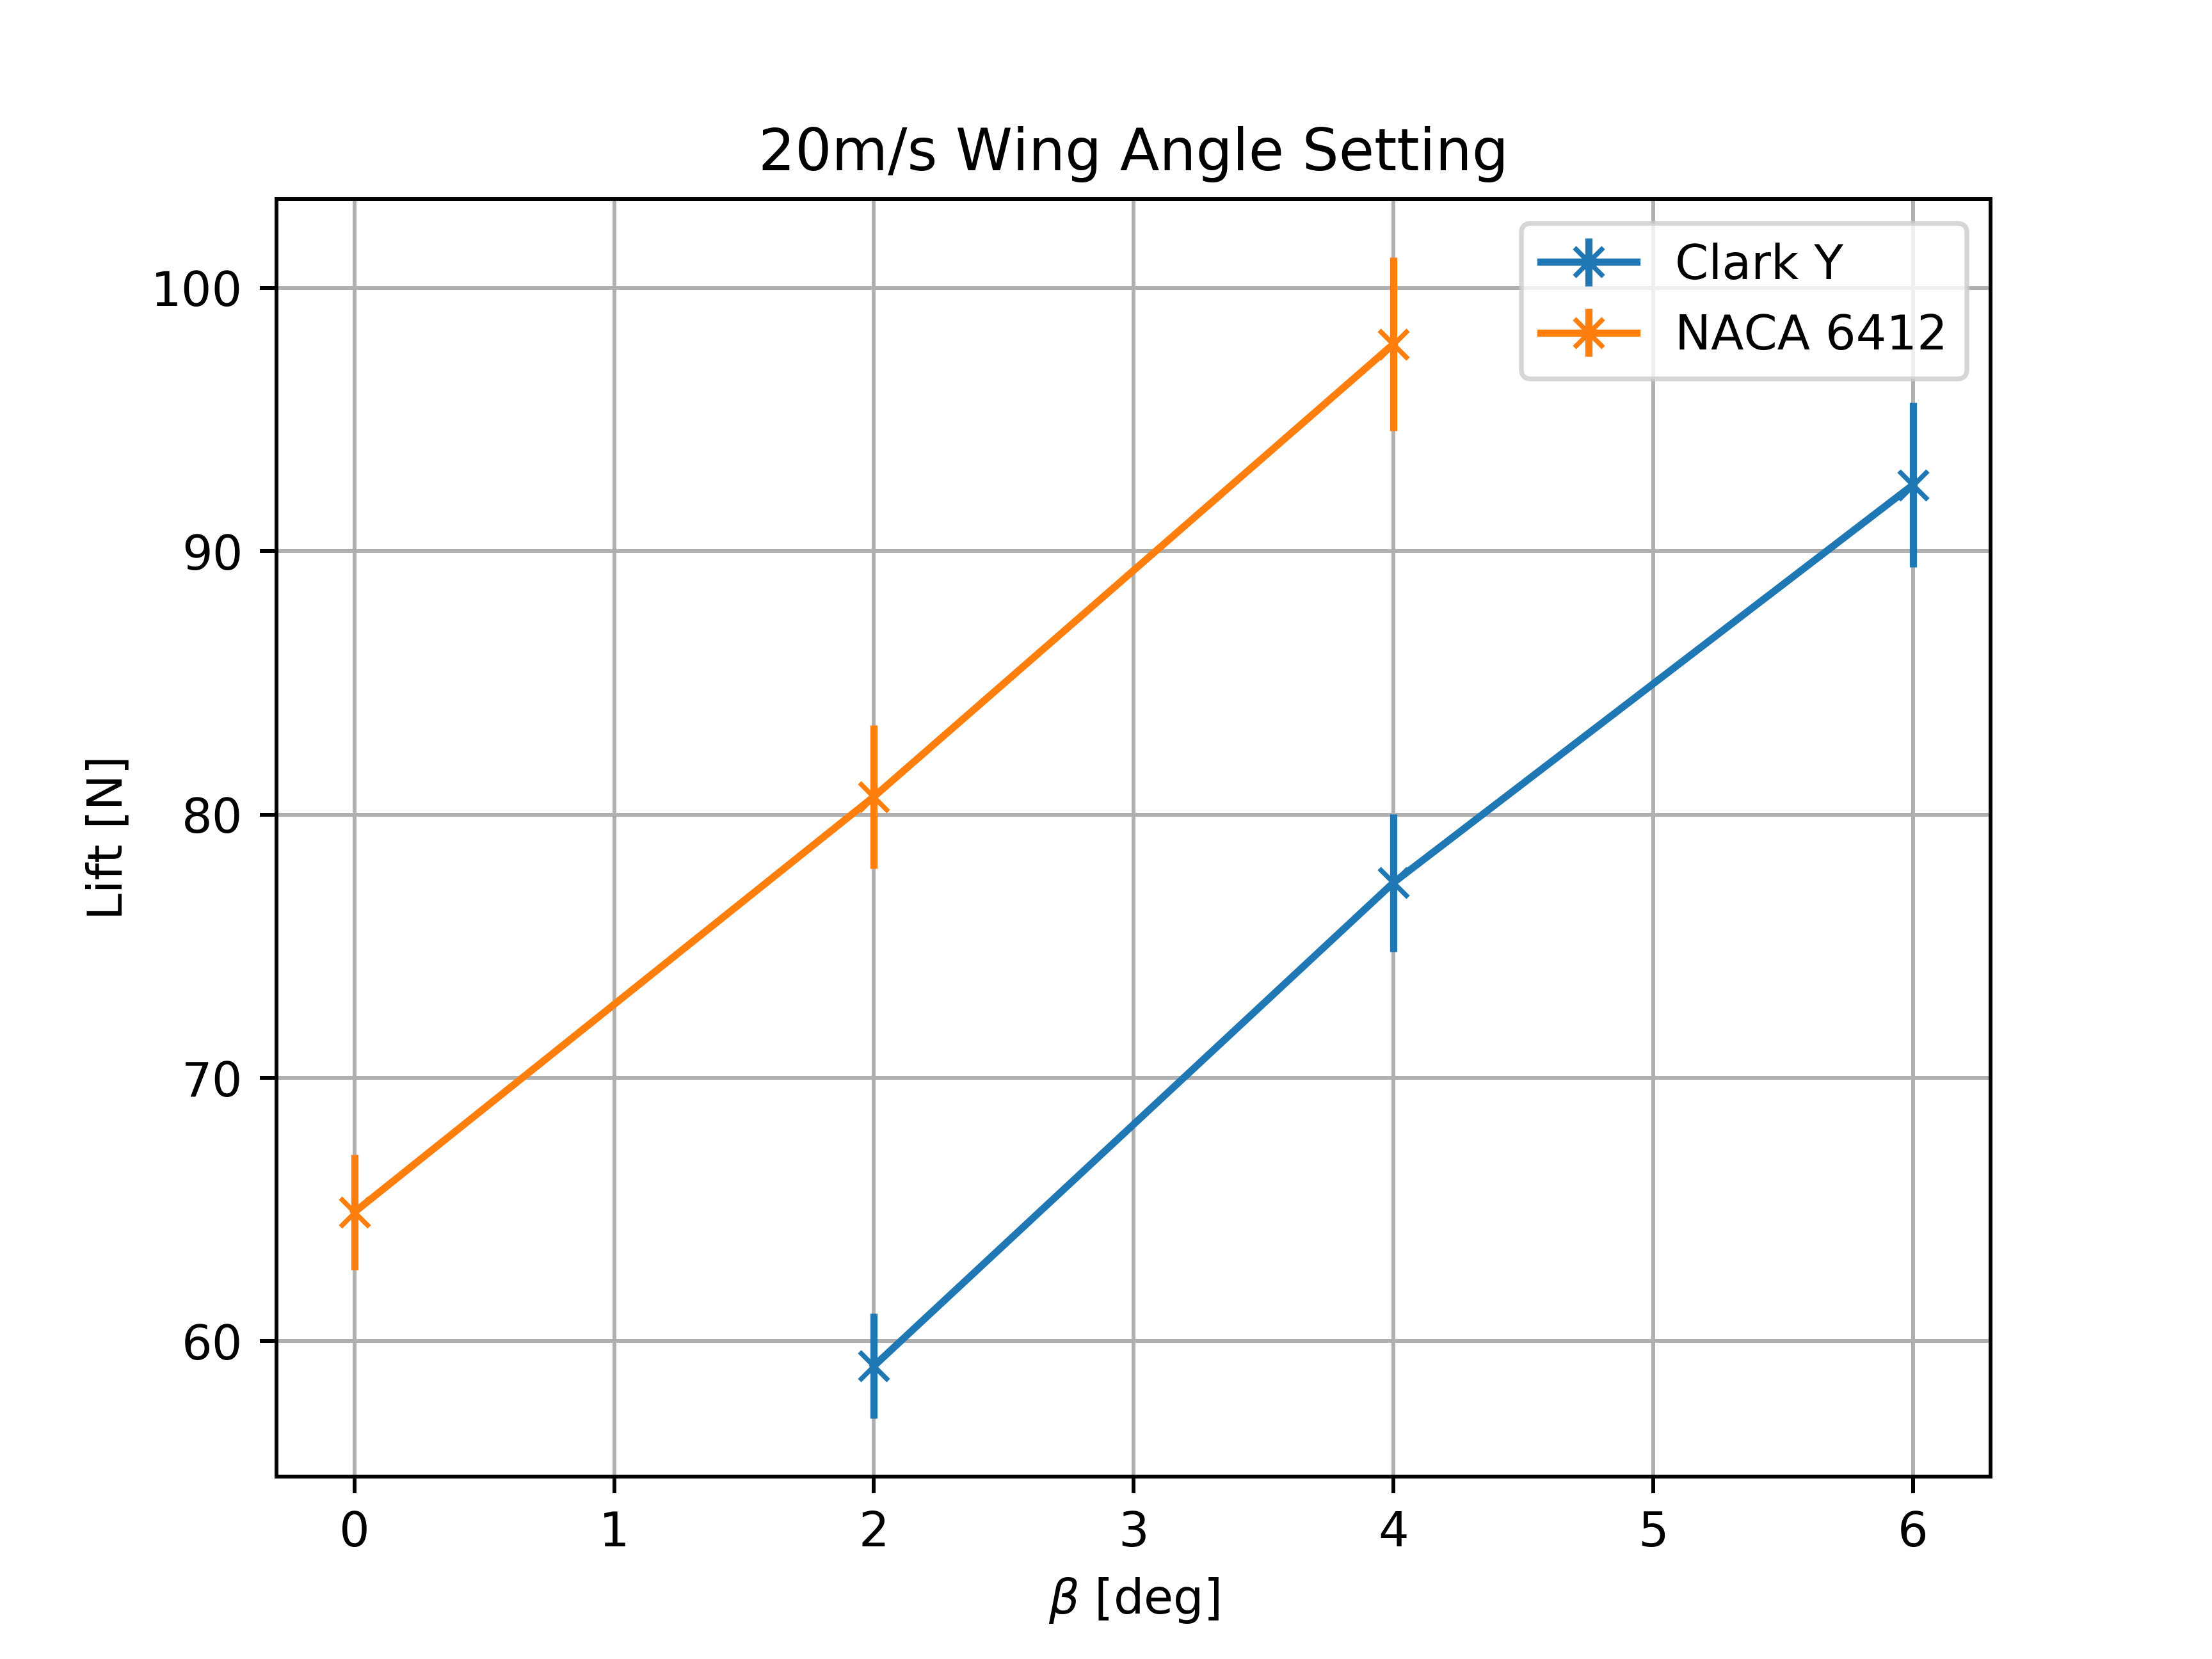
\includegraphics[width=\textwidth]{wing-setting-angle}
        \caption{Wing setting angle}
        \label{fig:wind-tunnel-results:wing-setting-angle}
    \end{subfigure}
    \begin{subfigure}[b]{\multiimagewidth\columnwidth}
        \centering
        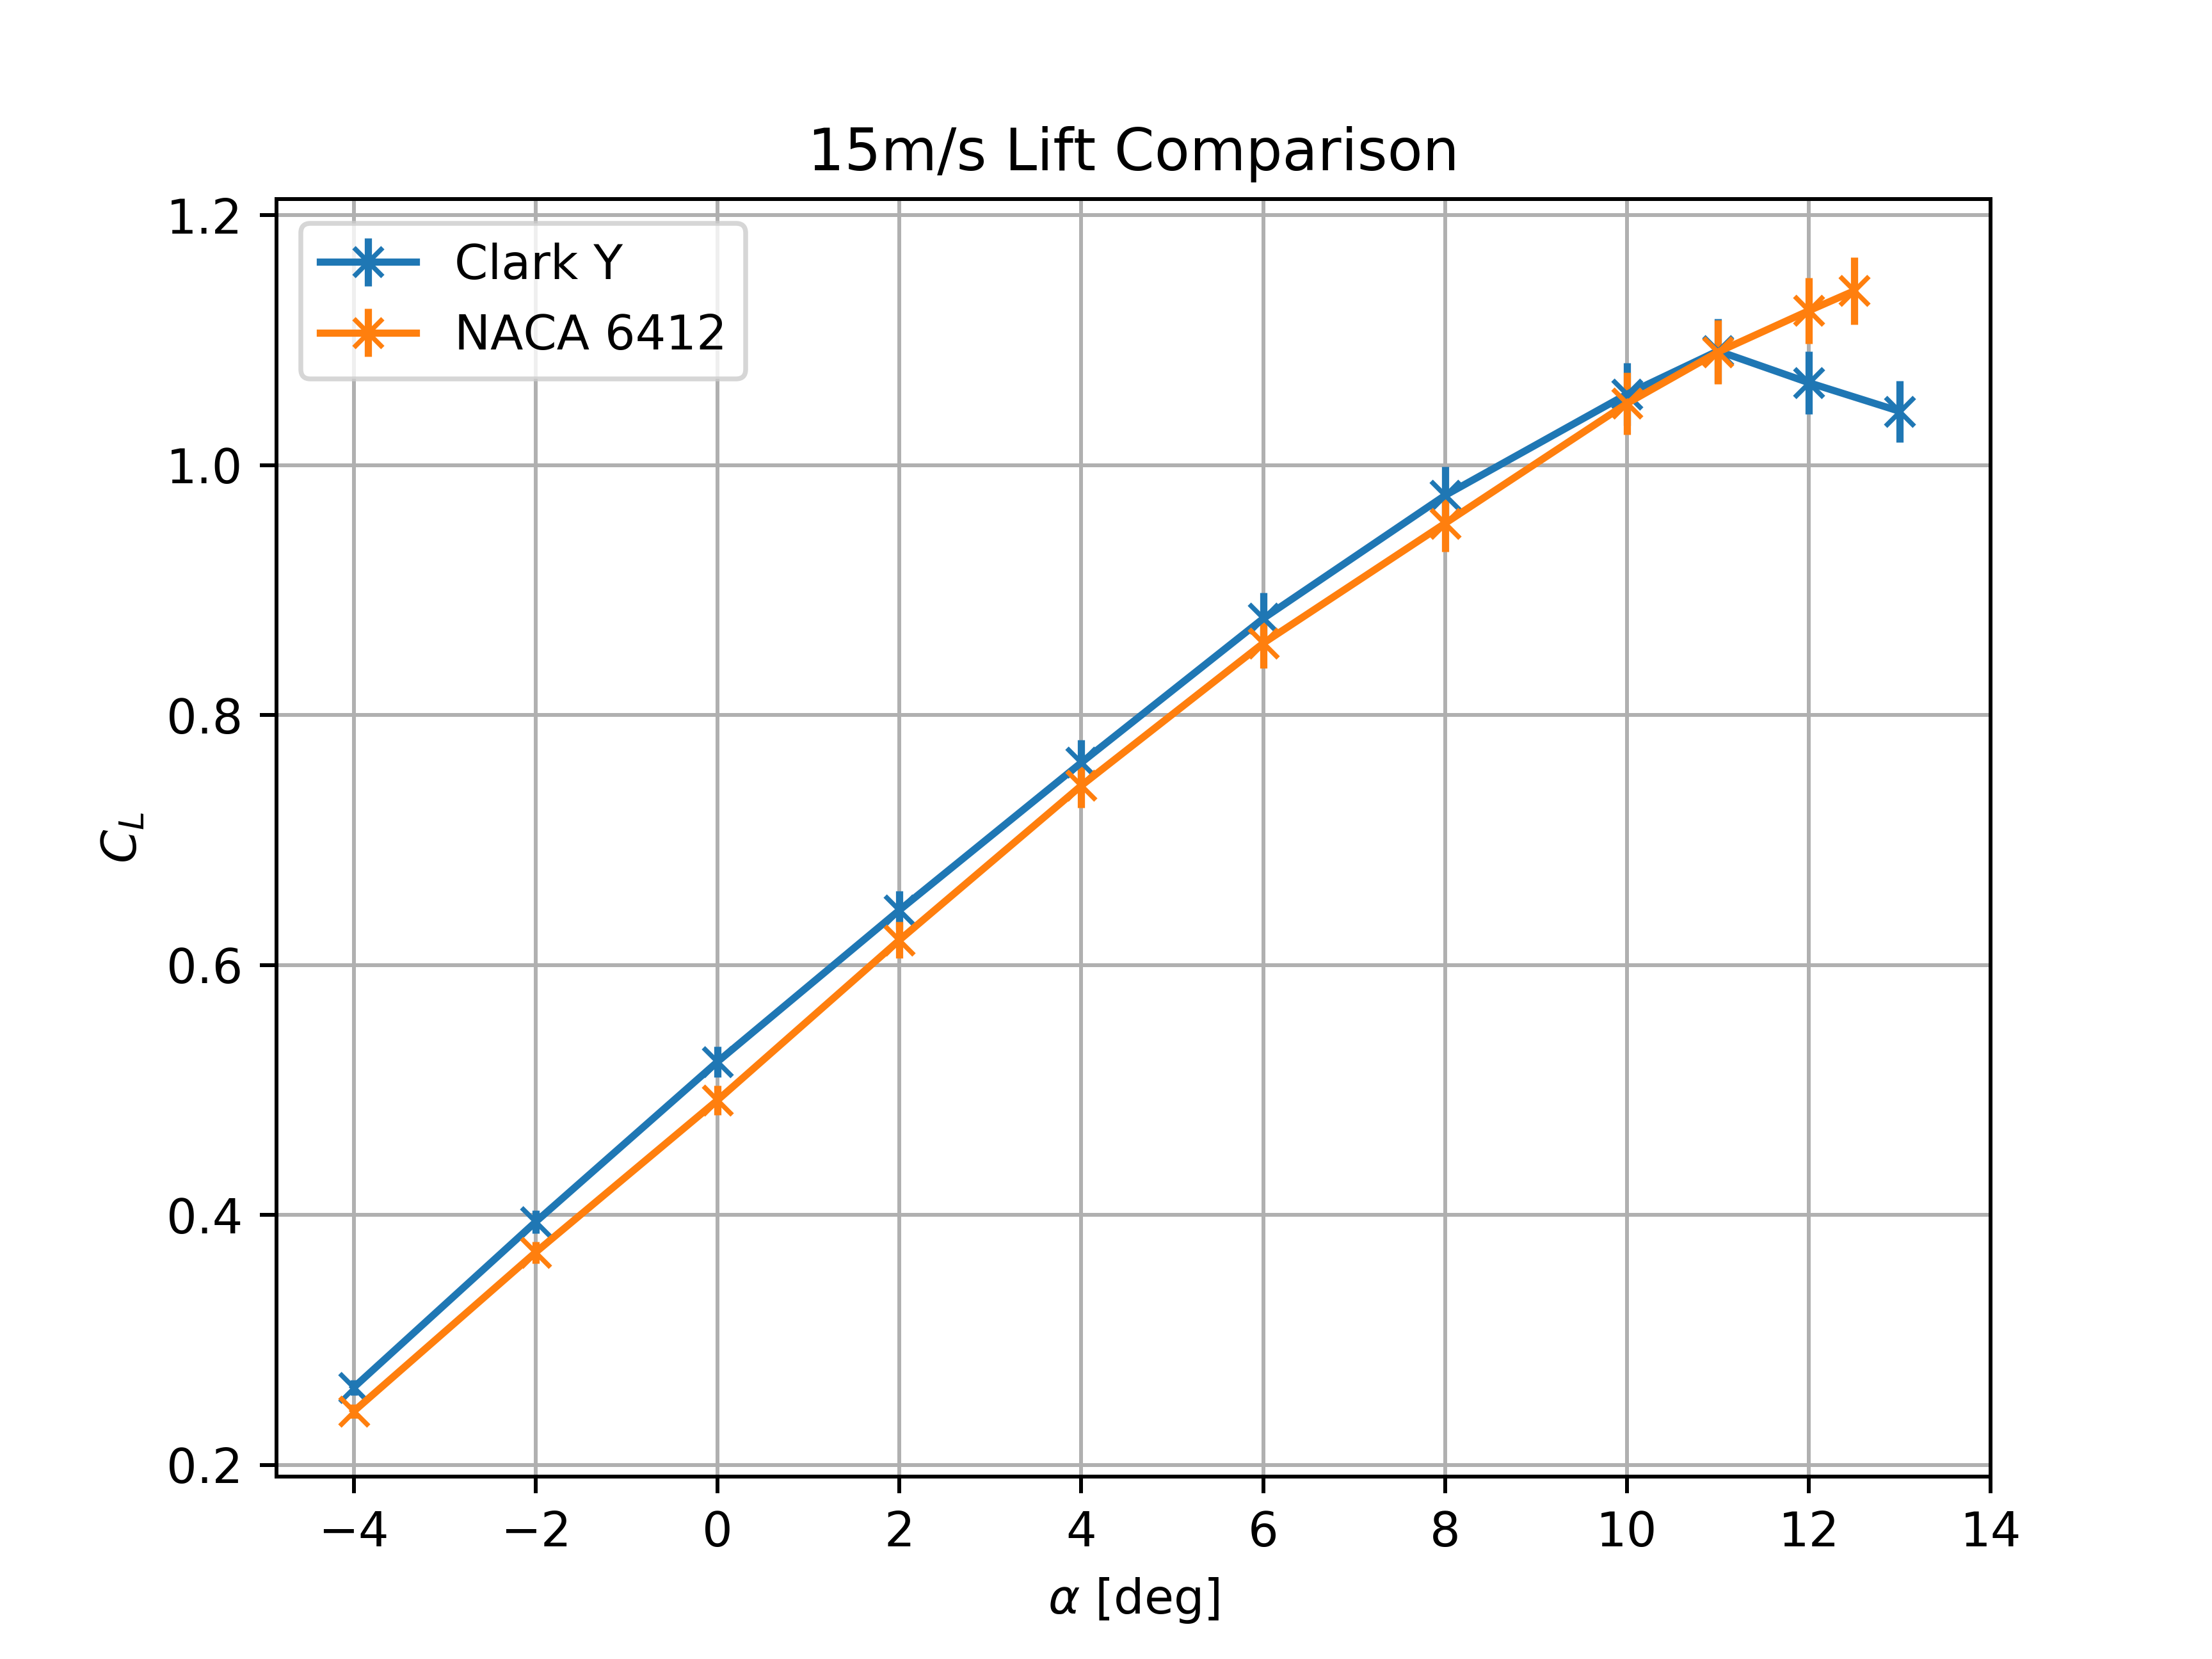
\includegraphics[width=\textwidth]{lift-comparison}
        \caption{Lift comparison}
        \label{fig:wind-tunnel-results:lift-comparison}
    \end{subfigure}

    \begin{subfigure}[b]{\multiimagewidth\columnwidth}
        \centering
        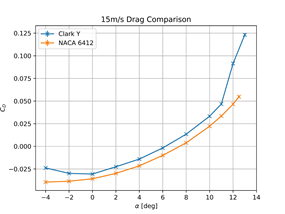
\includegraphics[width=\textwidth]{drag-comparison}
        \caption{Drag comparison}
        \label{fig:wind-tunnel-results:drag-comparison}
    \end{subfigure}
    \begin{subfigure}[b]{\multiimagewidth\columnwidth}
        \centering
        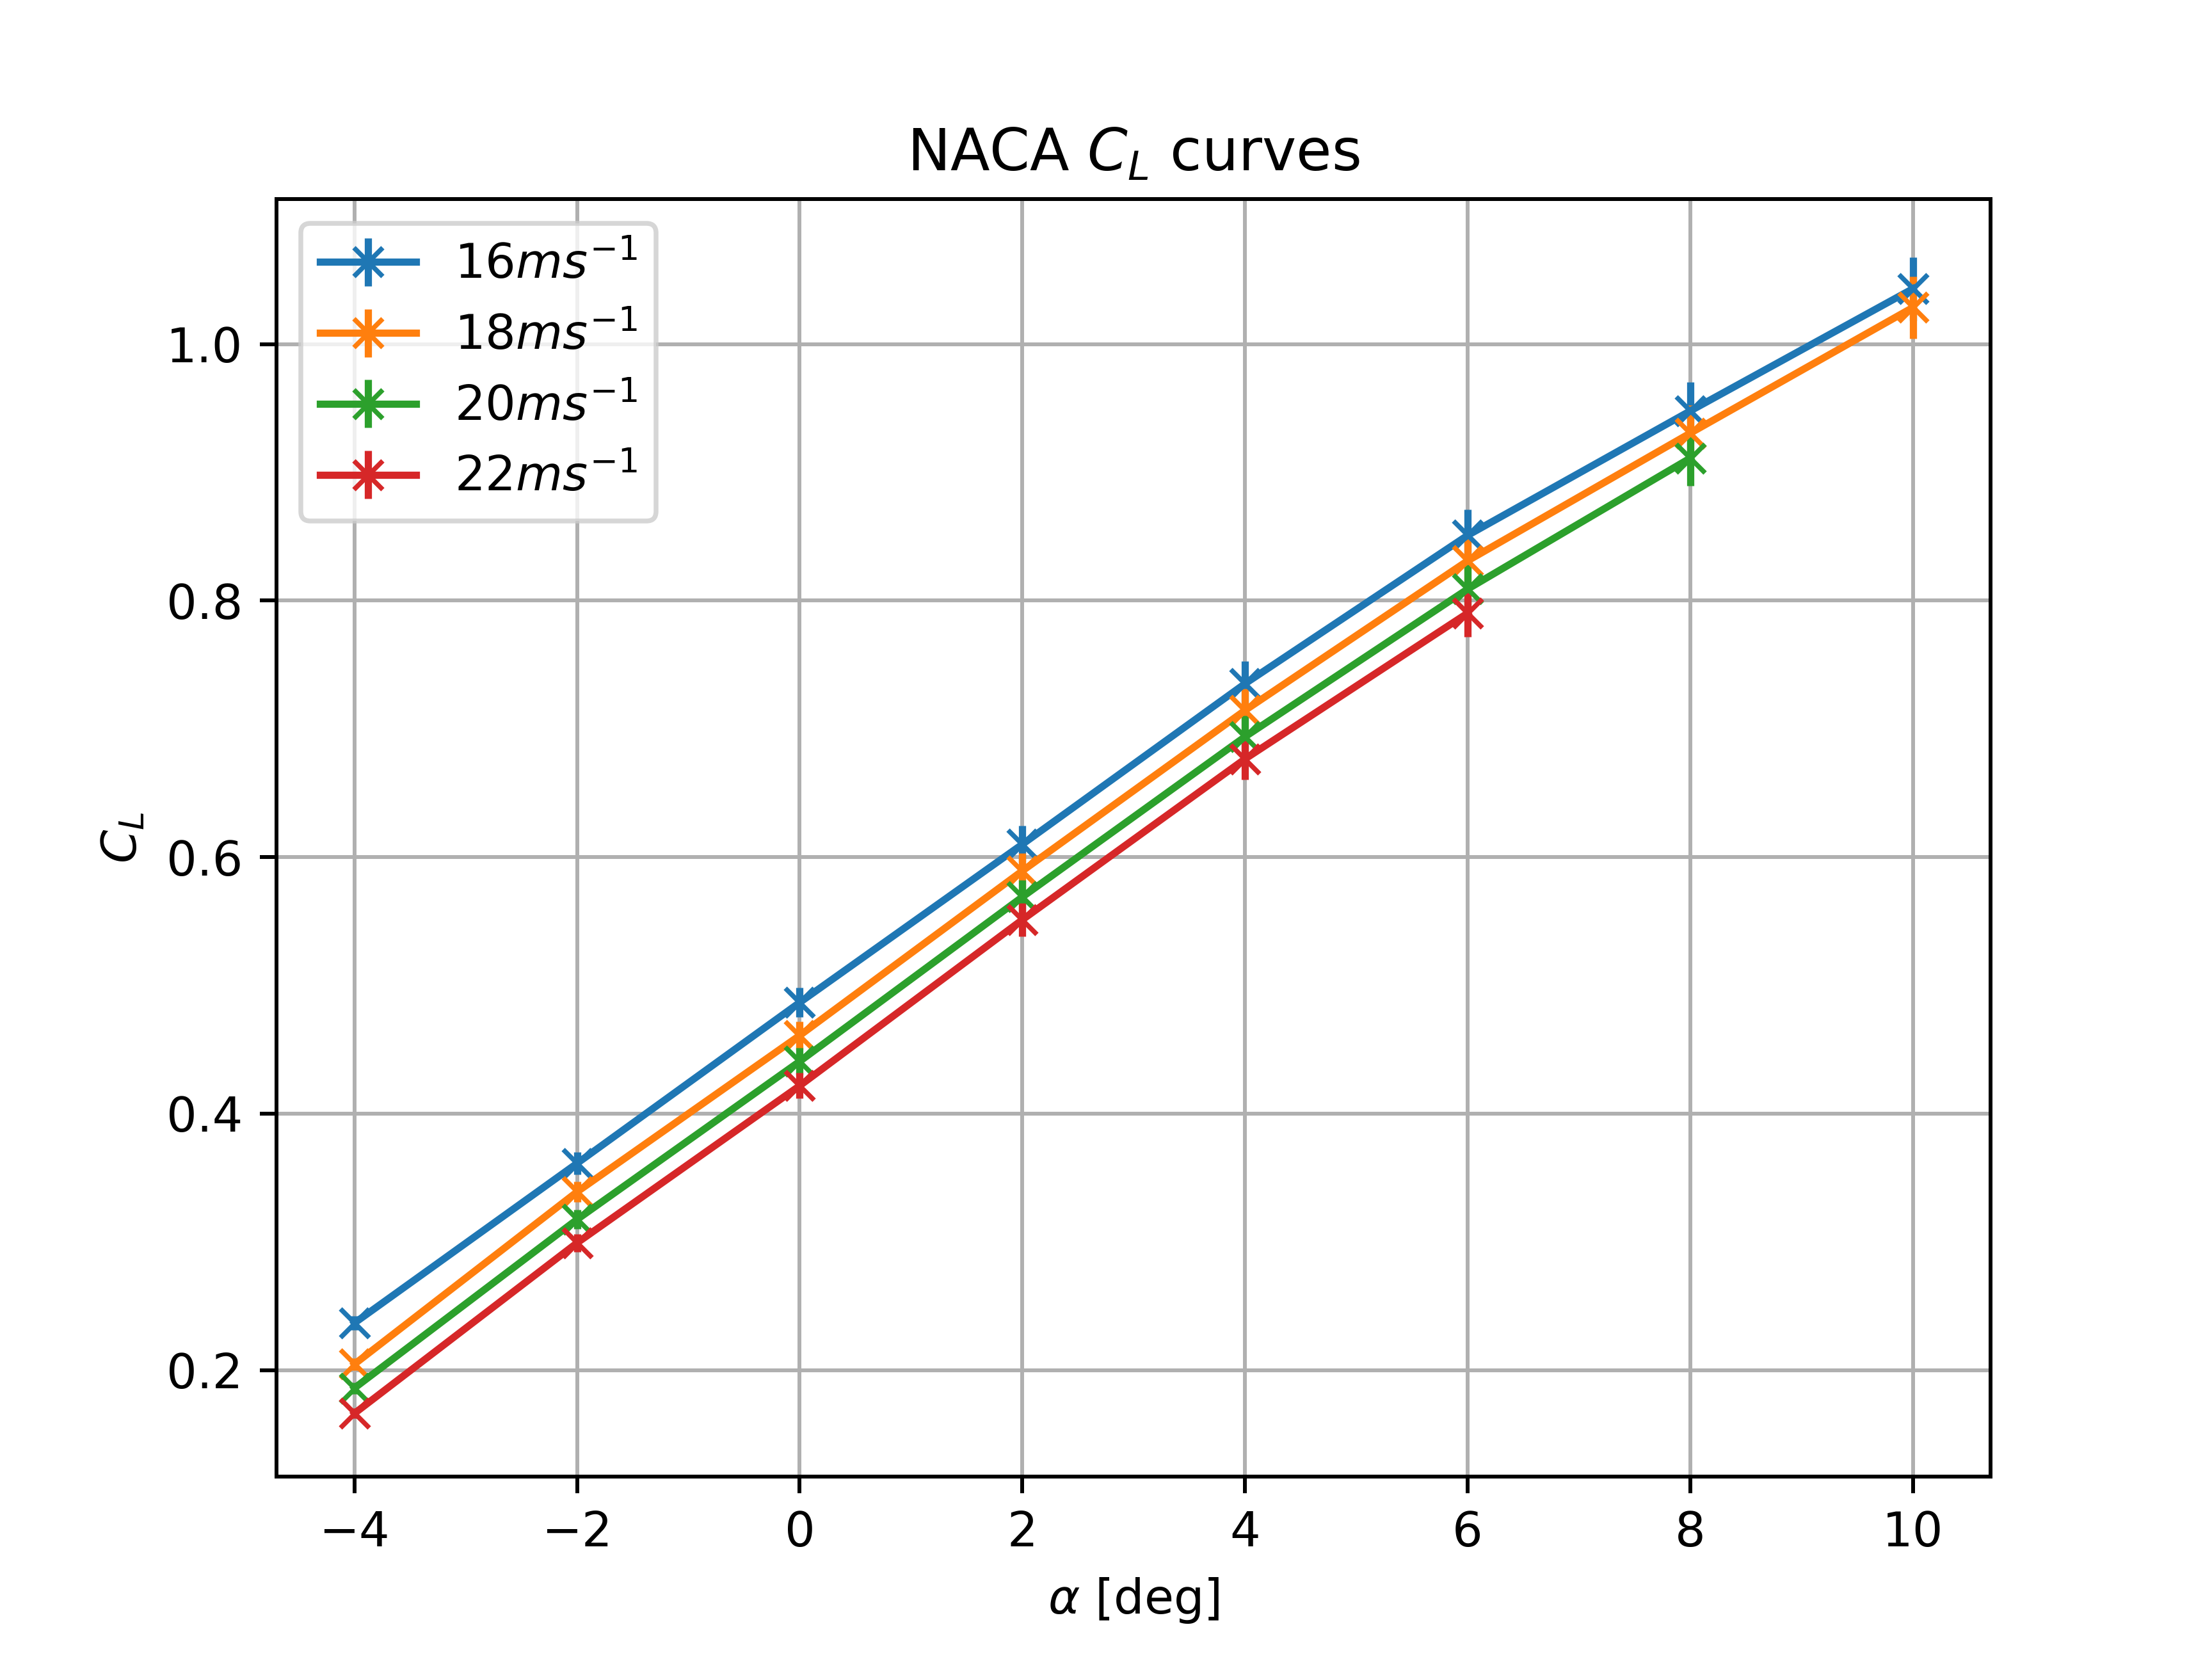
\includegraphics[width=\textwidth]{naca-lift-coefficient}
        \caption{NACA lift coefficient}
        \label{fig:wind-tunnel-results:naca-lift-coefficient}
    \end{subfigure}

    \begin{subfigure}[b]{\multiimagewidth\columnwidth}
        \centering
        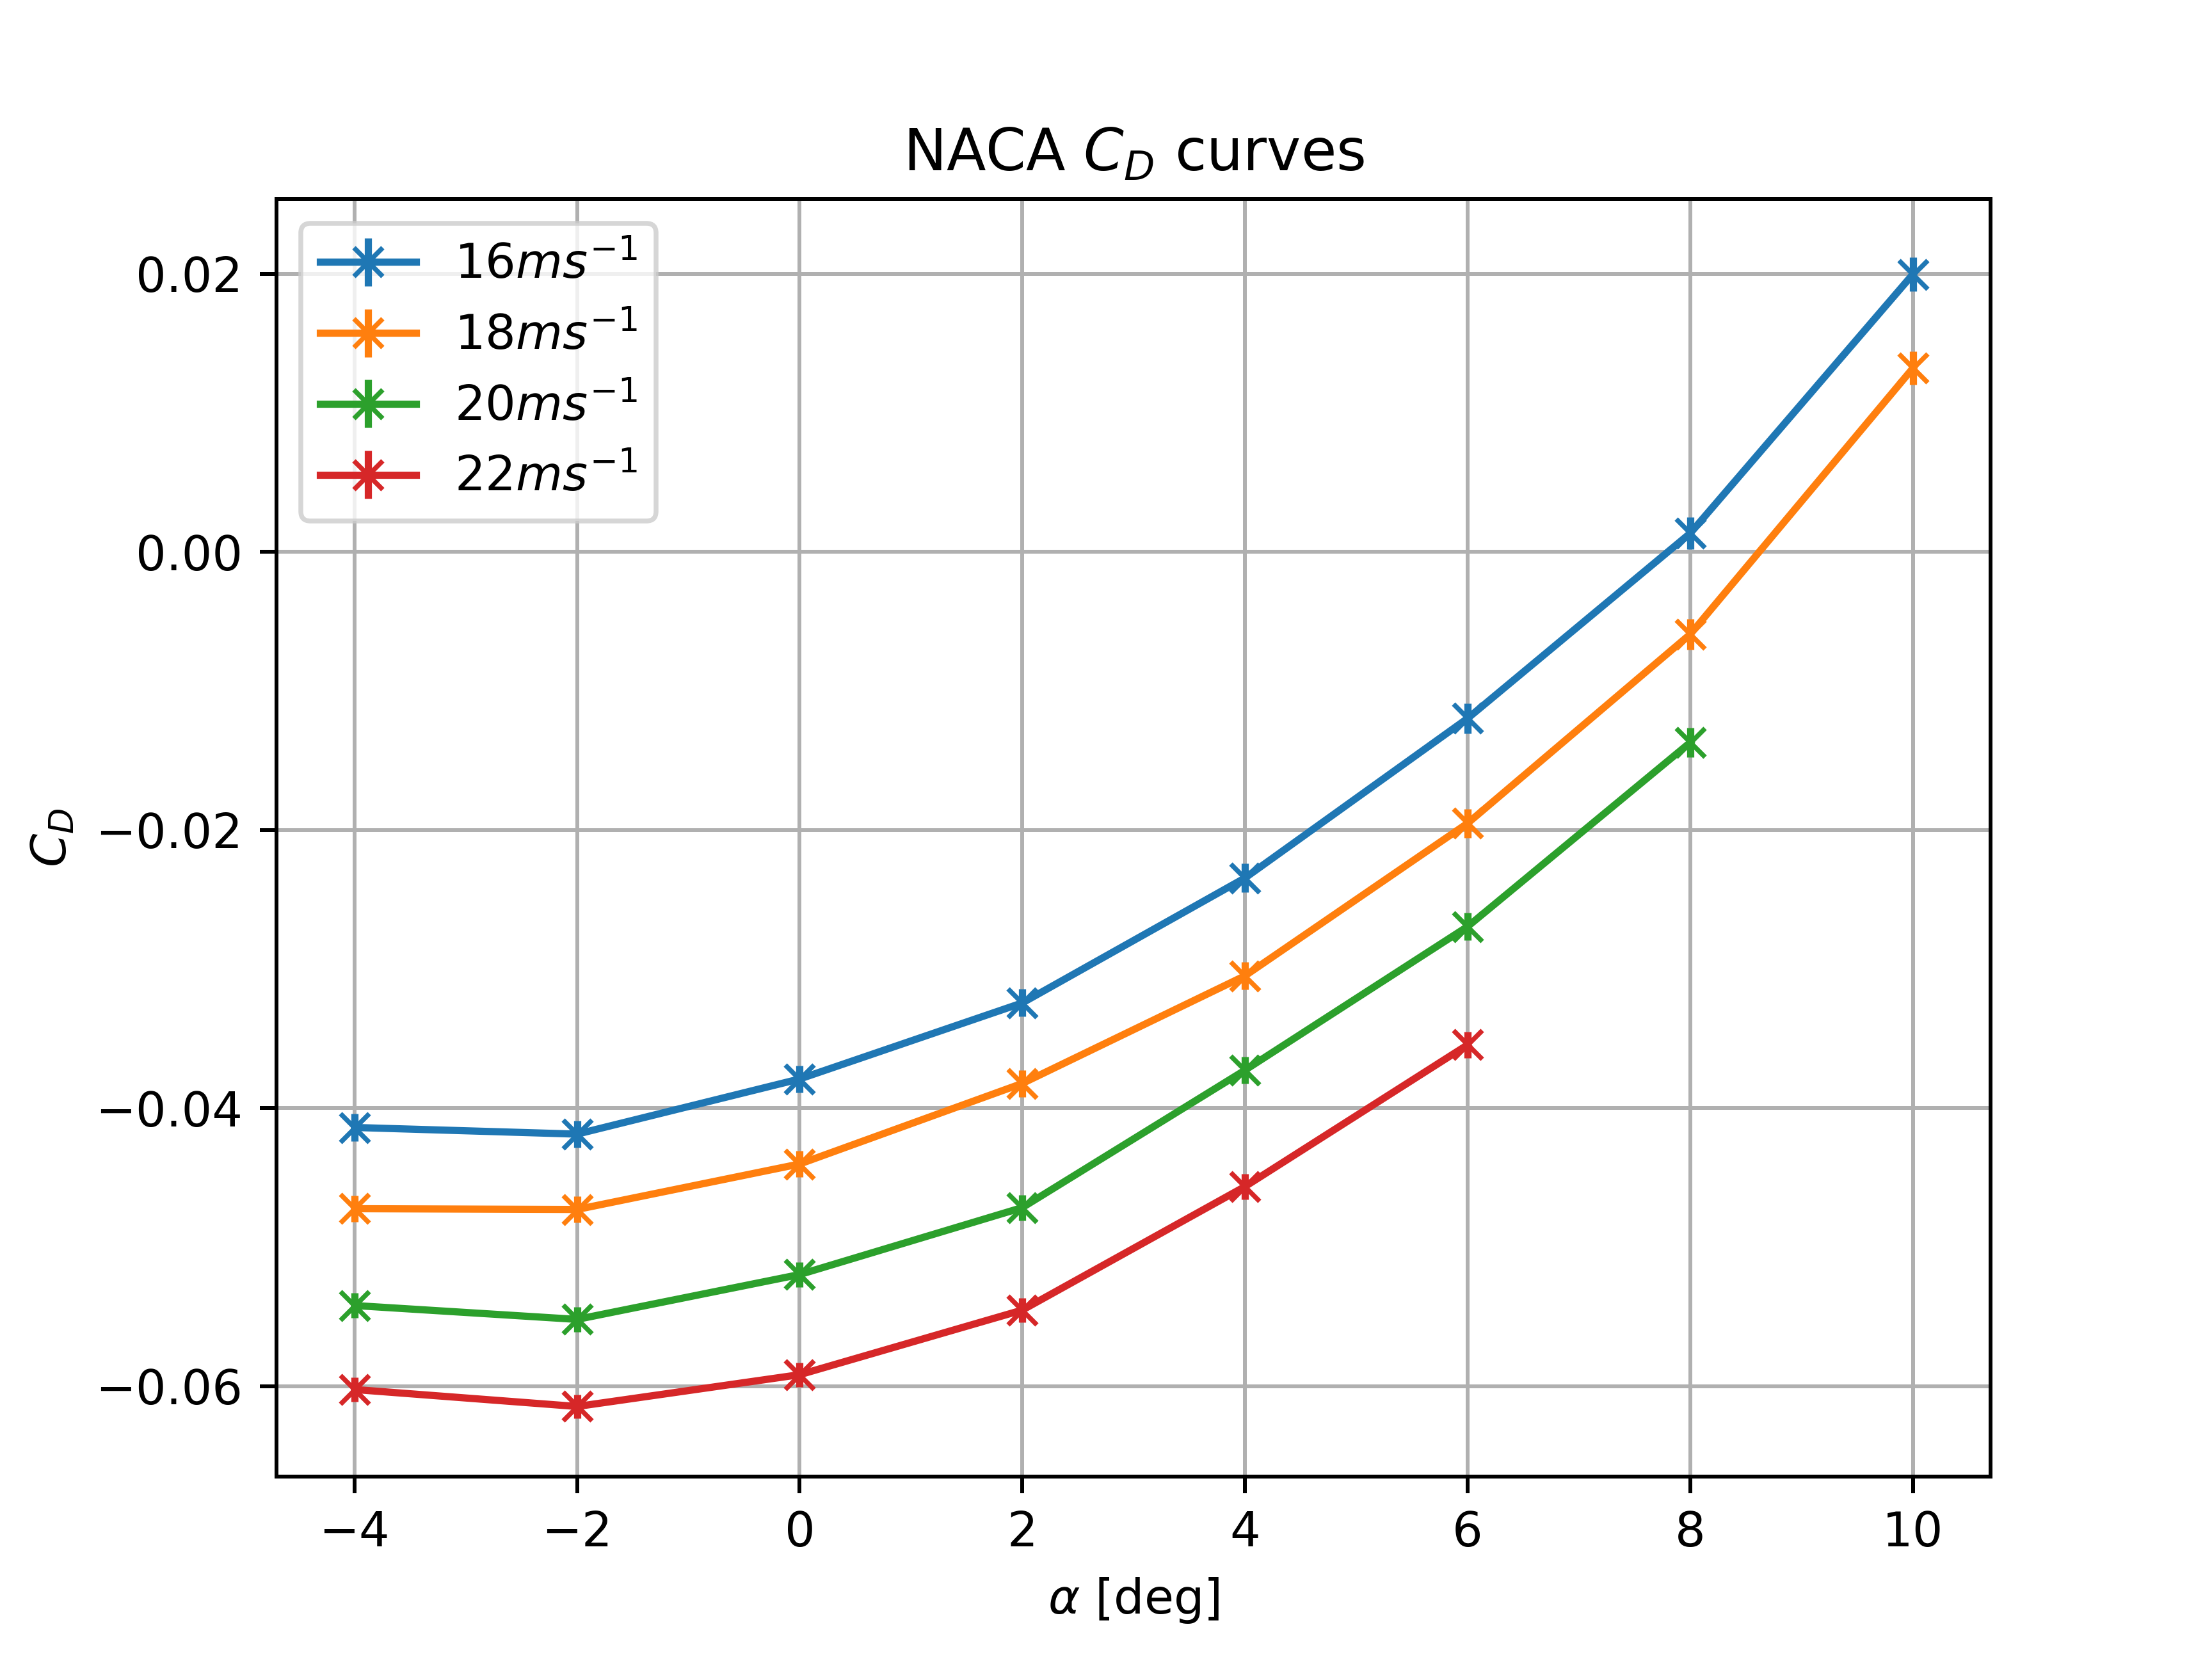
\includegraphics[width=\textwidth]{naca-drag-coefficient}
        \caption{NACA drag coefficient}
        \label{fig:wind-tunnel-results:naca-drag-coefficient}
    \end{subfigure}
    \begin{subfigure}[b]{\multiimagewidth\columnwidth}
        \centering
        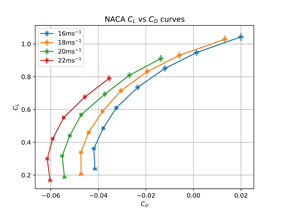
\includegraphics[width=\textwidth]{cl-against-cd}
        \caption{\cl\, against \cd}
        \label{fig:wind-tunnel-results:cl-against-cd}
    \end{subfigure}

    \begin{subfigure}[b]{\multiimagewidth\columnwidth}
        \centering
        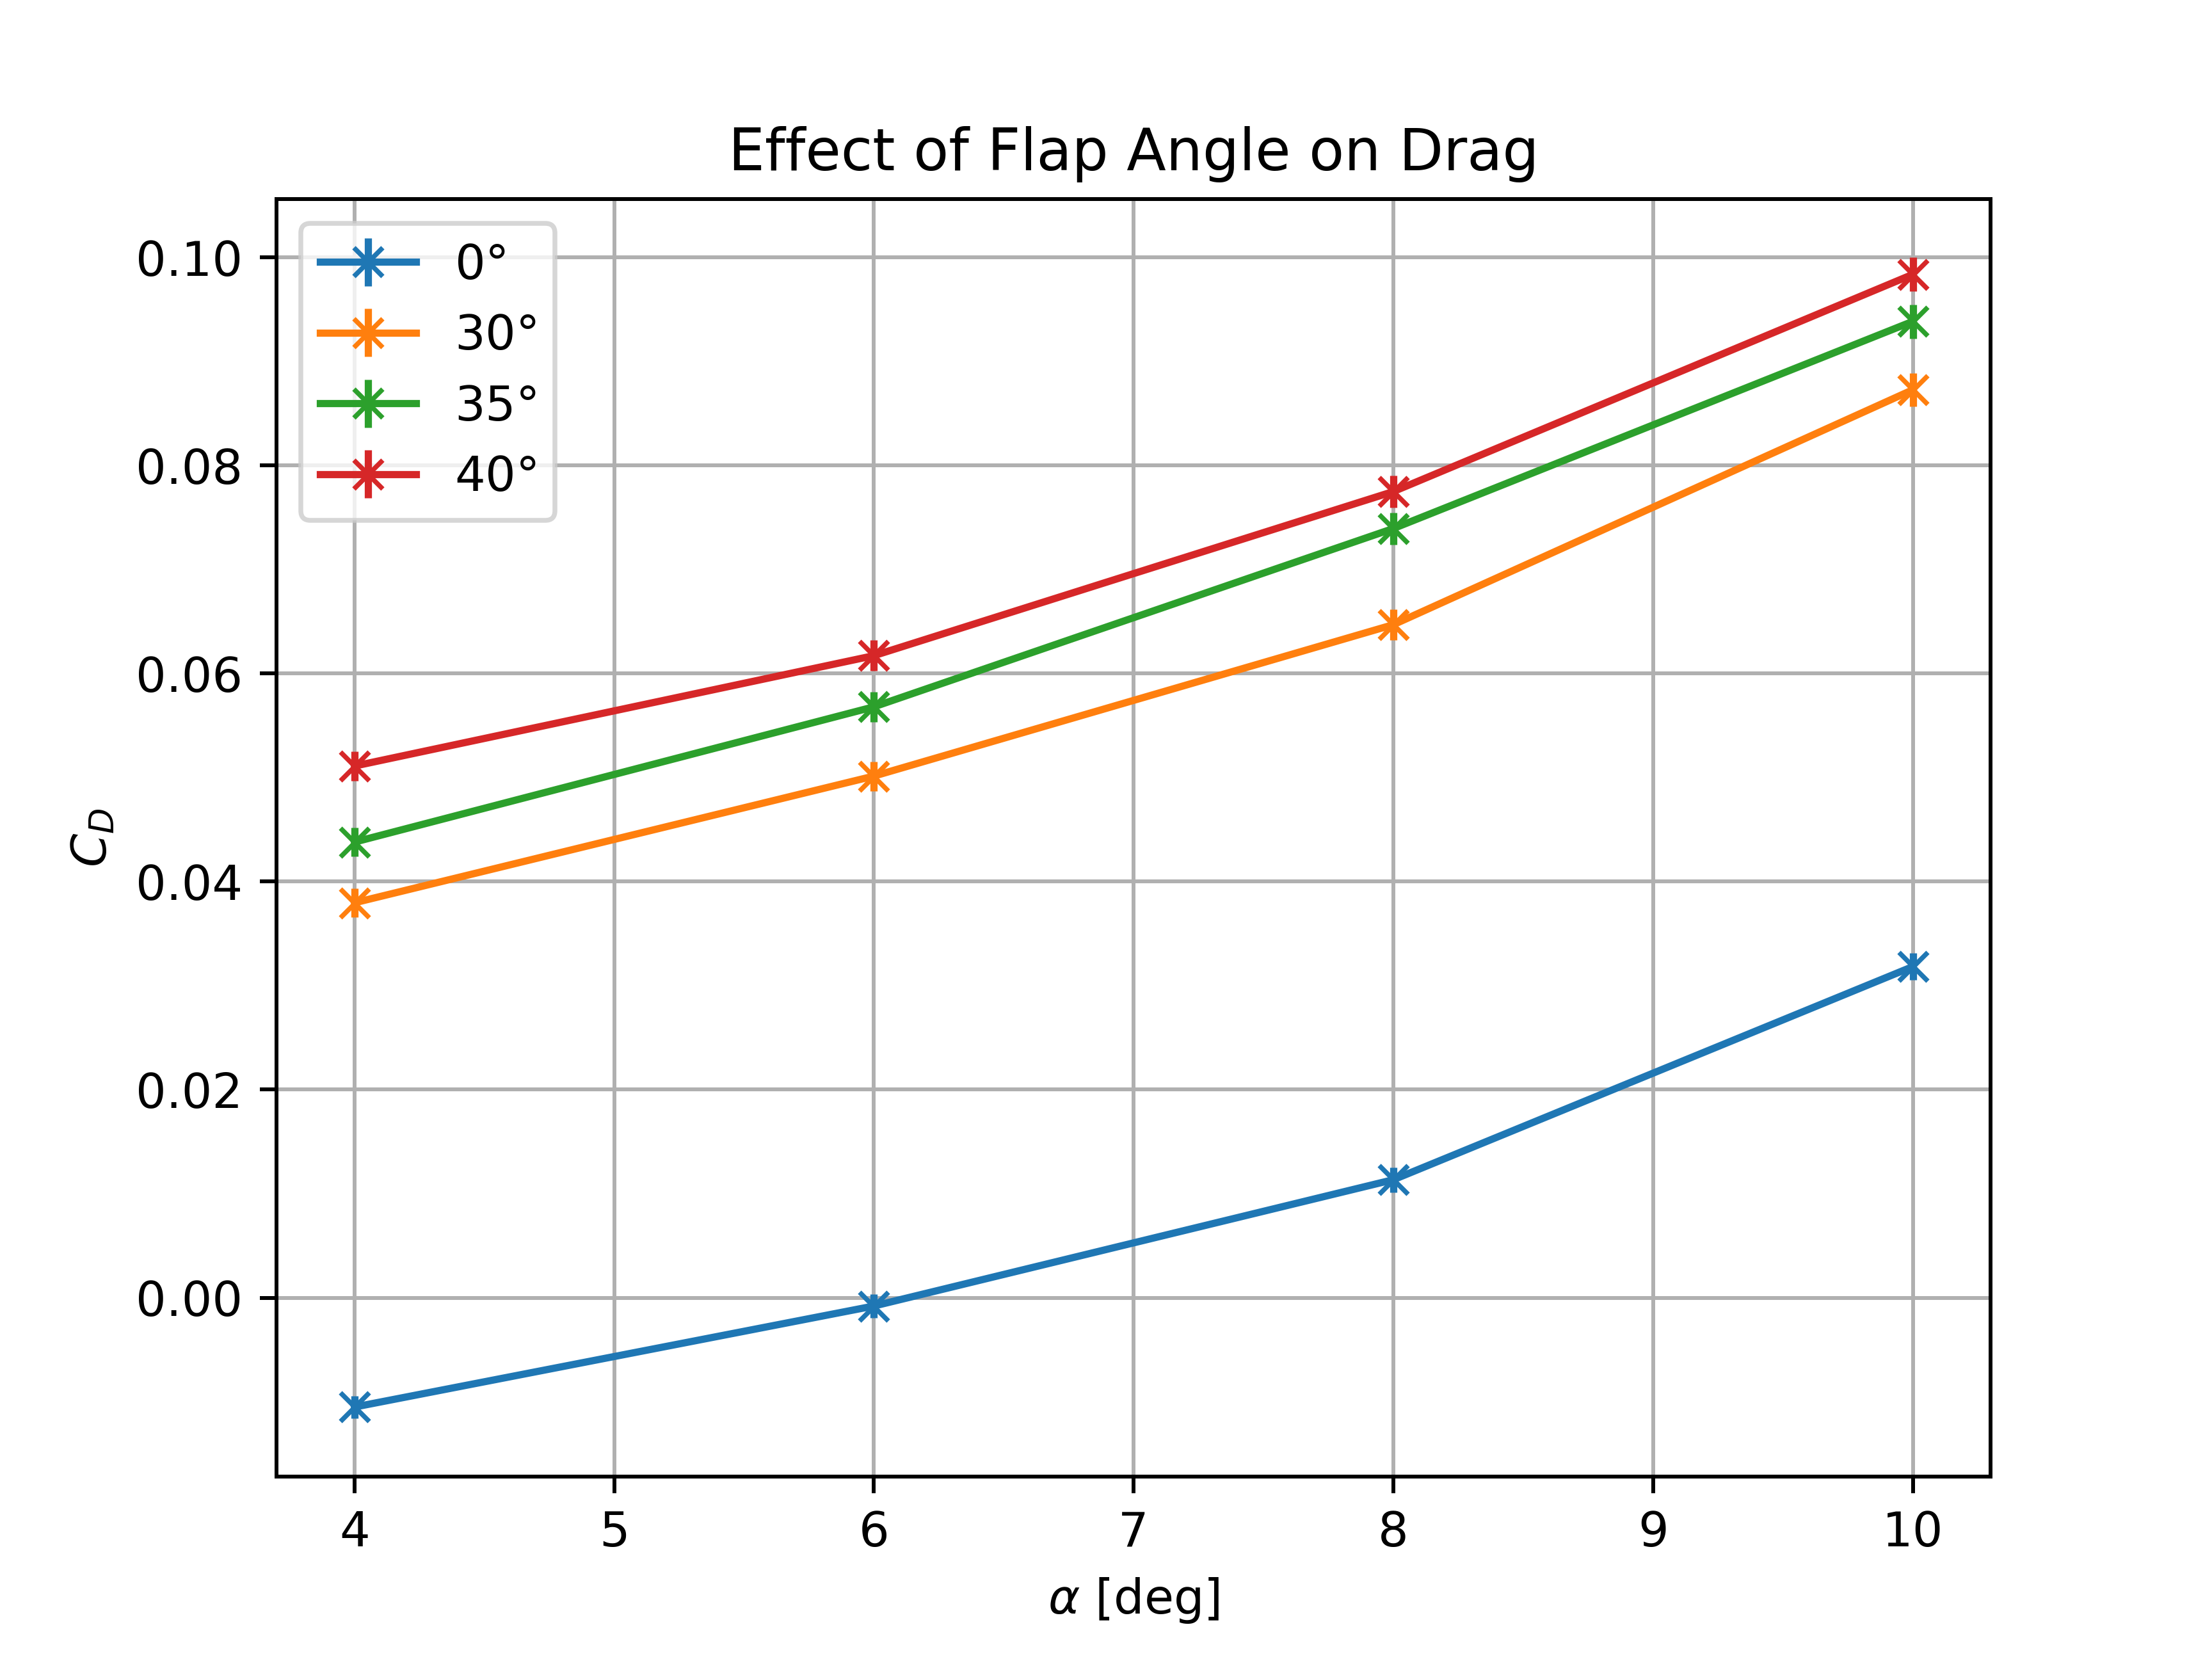
\includegraphics[width=\textwidth]{flap-drag-comparison}
        \caption{Flap drag comparison}
        \label{fig:wind-tunnel-results:flap-drag-comparison}
    \end{subfigure}
    \begin{subfigure}[b]{\multiimagewidth\columnwidth}
        \centering
        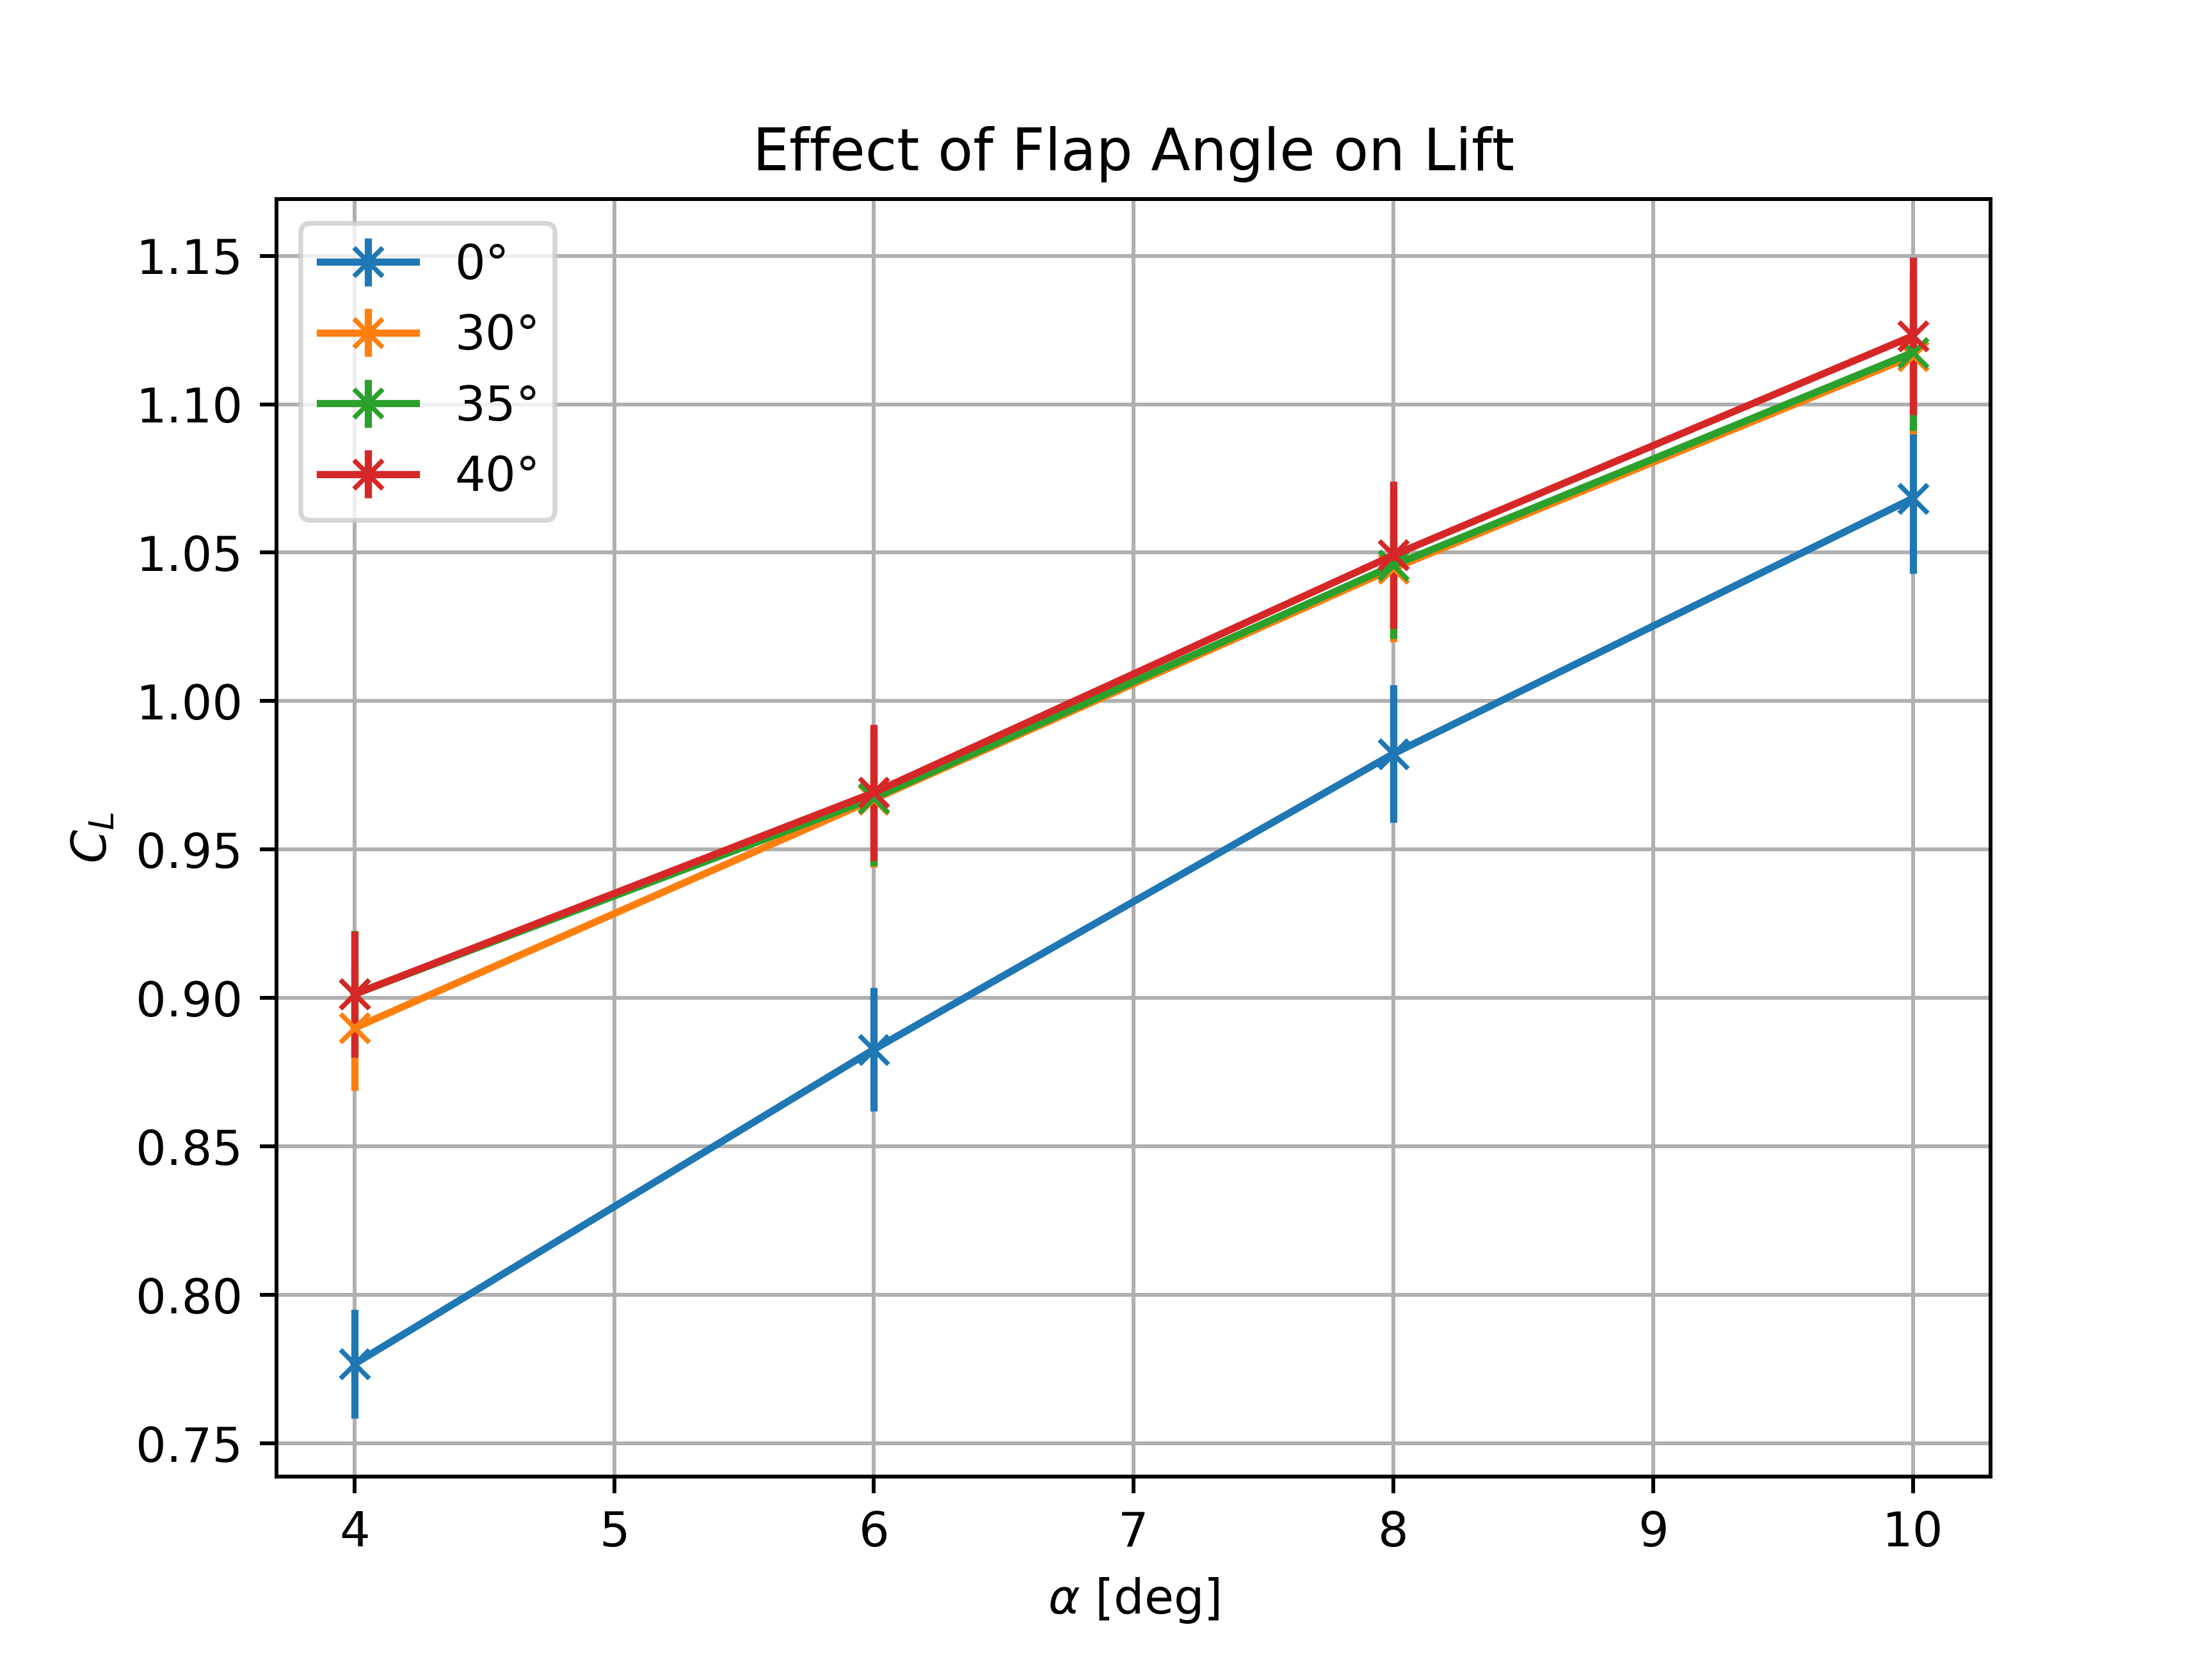
\includegraphics[width=\textwidth]{flap-lift-comparison}
        \caption{Flap lift comparison}
        \label{fig:wind-tunnel-results:flap-lift-comparison}
    \end{subfigure}

    \begin{subfigure}[b]{\multiimagewidth\columnwidth}
        \centering
        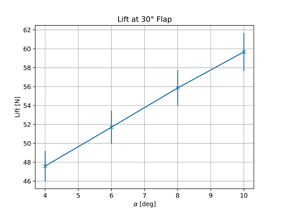
\includegraphics[width=\textwidth]{30-degree-flap-lift}
        \caption{30$^o$ flap lift}
        \label{fig:wind-tunnel-results:30-degree-flap-lift}
    \end{subfigure}
    \begin{subfigure}[b]{\multiimagewidth\columnwidth}
        \centering
        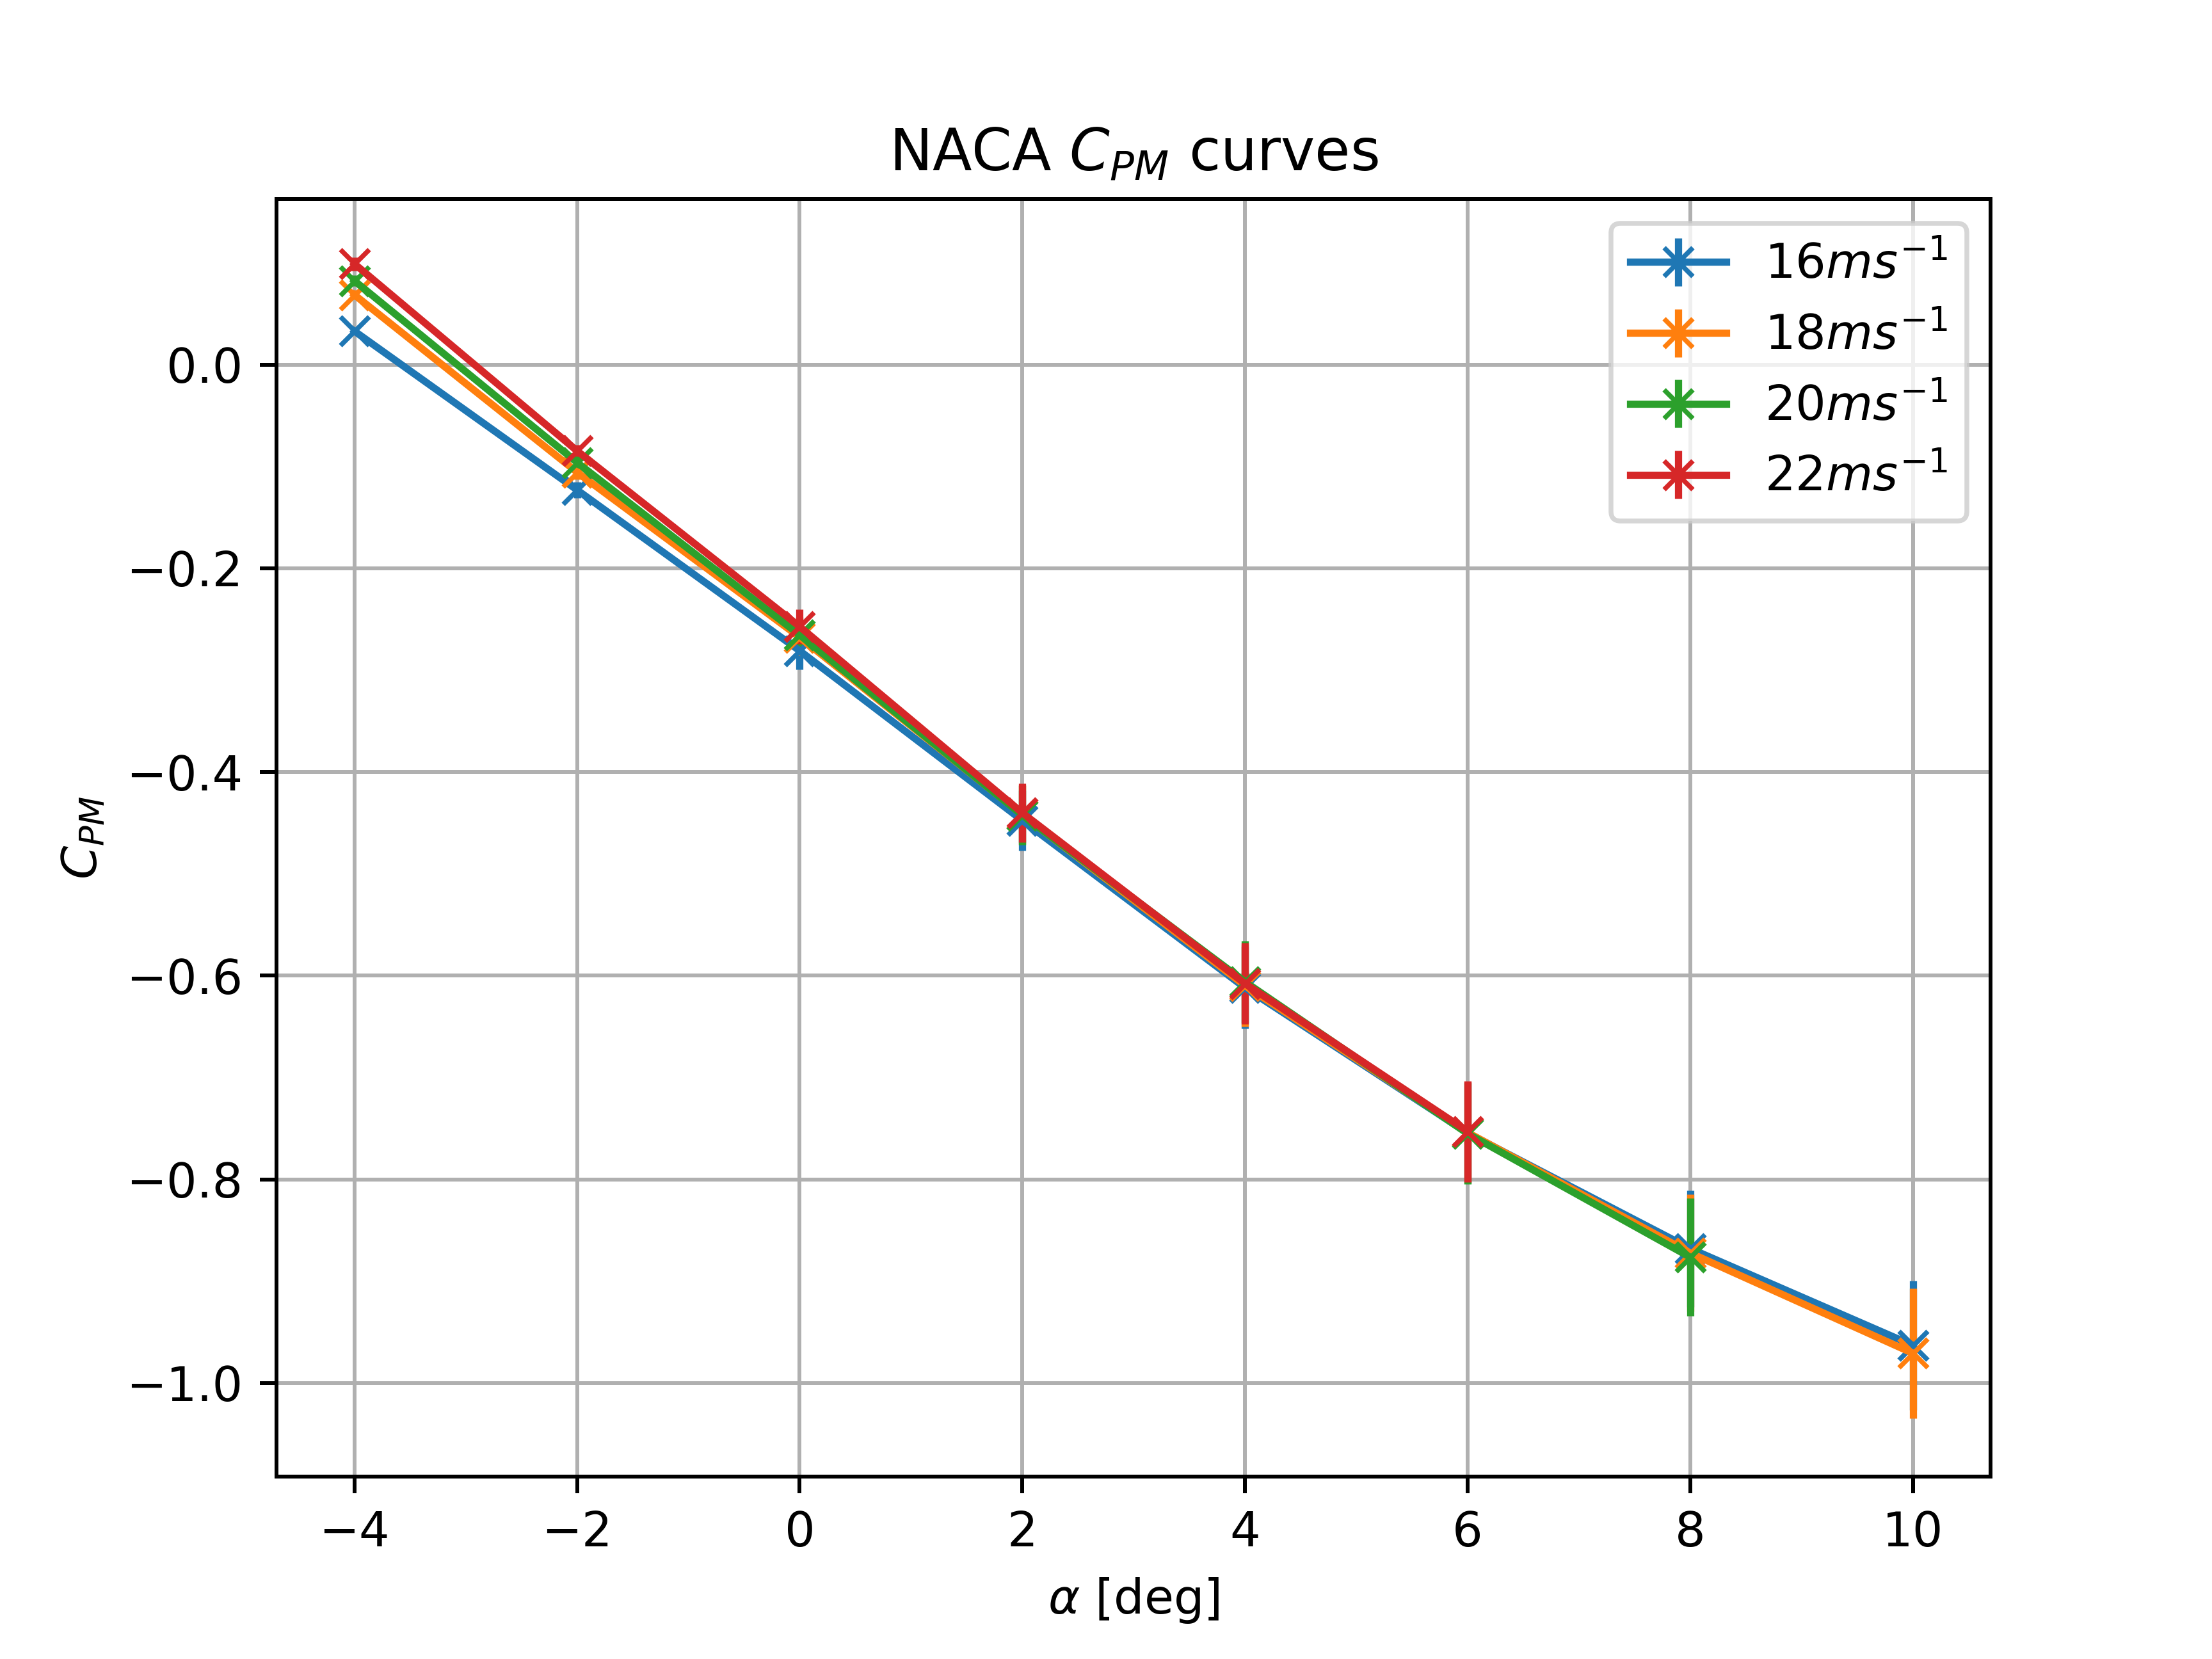
\includegraphics[width=\textwidth]{moment-coefficients}
        \caption{Moment coefficients}
        \label{fig:wind-tunnel-results:moment-coefficients}
    \end{subfigure}

    \caption{graphical results of the analysis of data gathered during the wind tunnel test.}
    \label{fig:wind-tunnel-results}
\end{figure}

The uncertainty of the results was calculated and is shown as vertical bars for every point on the plots in Figure \ref{fig:wind-tunnel-results}.
The uncertainties were calculated using the known accuracies of the recorded results, as well as repeats performed during the testing.
The maximum number of repeats for one test was only two, and so while the sample size is not significant, the uncertainties are still reasonably small even with a \pc{95.45} confidence.
These uncertainties were then converted to percentages and applied to all results of that type, with an example table for the uncertainty of \cl\, shown in Table \ref{tbl:cl-uncertainty}, and the others provided in Appendix \ref{appendix:uncertainty-analysis-tables}.

% TODO: units
% TODO: define uncertainty and variance outside table
% TODO: reduce width slightly
\importtable{|
    >{\raggedright\arraybackslash}m{0.16\columnwidth}
    >{\raggedleft\arraybackslash}m{0.16\columnwidth}
    >{\raggedleft\arraybackslash}m{0.17\columnwidth}
    >{\raggedleft\arraybackslash}m{0.17\columnwidth}
    >{\raggedleft\arraybackslash}m{0.17\columnwidth} |
}{
    \hline
    Measured variable & $L$ & $q$ & $S$ & Rep. \cl \\
    \hline
    Typical value & 77.04 & 249.55 & 0.6 & 0.01715 \\
    Accuracy & 0.07704 & 0.349 & 0.0012 & 0.01213 \\
    PDF & rect. & rect. & rect. & norm. \\
    PDF factor & 1.7321 & 1.7321 & 1.7321 & 1 \\
    $k$ factor & 1 & 1 & 1 & 1 \\
    SC value & 0.006679 & -0.00206 & -0.85754 & 1 \\
    Uncertainty & 0.000297 & -0.000416 & -0.000594 & 0.012128 \\
    Variance & $9\times10^{-8}$ & $1.7\times10^{-7}$ & $3.5\times10^{-7}$ & $1.471\times10^{-4}$ \\
    \hline
}{uncertainty calculations for \cl; the uncertainty and variance rows refer to the value of uncertainty and its variance in each measured variable.}{cl-uncertainty}

\importtable{| l r |}{
    \hline
    Combined standard uncertainty & 0.01215 \\
    \cl\, mean & 0.5145 \\
    Percentage uncertainty & 2.36 \\
    \hline
}{uncertainty summary for \cl.}{uncertainty-summary}

Unfortunately, the scope of the work required to design a fully functional tailplane with control surfaces had not yet been realised, and the design was far too simple, with no mounting angle or control surfaces.
The tail was also undersized, as observed by the project supervisors.
Because of this, little work went into analysing the results from this test in terms of the tailplane, and work on the next version essentially started from scratch. 

\subsection{Motor and propellor test} \label{sec:design-process:interim-design-review:motor-and-propellor-test}

\subsubsection{Overview} \label{sec:design-process:interim-design-review:motor-and-propellor-test:overview}

\importimage{motor-bracket}{the motor bracket attached to the rear of the motor.}{Motor bracket}{0.5}
\importimage{motor-test}{the motor in the wind tunnel.}{Motor test}{0.5}

Once the motor and propeller selection had been completed based on wind tunnel results and propeller performance analysis (\ref{sec:design-process:preliminary-design:propulsion:sizing}), one of the wing motors was ordered with its tractor configuration propeller in order to test them together.
This test was to be performed in a small wind tunnel so as to give data for the motor in flight as well as a static thrust test.
The motor mount was a load cell located at the centre of the wind tunnel section, as shown in Figure \ref{fig:motor-test}, and to attach the motor a bracket was required.
The main part of this bracket had already been made for the testing of a different motor by the university, and so only a small plate was required to mount the purchased motor to the existing setup.
This mount was made from aluminium sheet to fit to the back of the motor and mount onto the load cell, and is shown in Figure \ref{fig:motor-bracket}.
It required some precision marking and drilling for the outer holes as there were tight tolerances on the bracket to which it was to attach, while the motor holes could be slightly less precise due to the countersunk bolts holding it in place.
A central clearance hole was required to allow the motor shaft to pass through into the void created by the existing bracket, to avoid the motor shaft hitting the load cell.

The tests carried out were at wind speeds of \mps{0}, \mps{10}, and \mps{15}, and at each wind speed the voltage was held at around \volts{14.85} +/- \volts{0.05} $-$ representing a partially drained battery $-$ and the current was varied from \amps{0} to \amps{22}, giving a range of RPM at which the thrust and torque data were collected, up to a maximum power of \watts{330}.
The RPM was measured from the input to the motor, rather than directly from the blades, because the blades of the propeller were too short to reach in front of the laser.
Nevertheless, this RPM data was accurate to within 100RPM which was adequate for this experiment.

The load cell used to mount the motor formed a blockage in the wake of the propeller, and so while this will have affected the results, the effect of this was minimised by minimising the size of the manufactured bracket.
Furthermore, the motor $-$ when attached to the model $-$ would have the blockage of the wing and the power unit housing behind it, so this effect could be a good representation of the motor in flight.
In order to maximise the performance of the propeller, it was sanded before the test to remove any manufacturing defects and to ensure a smooth surface for the airflow.
The propeller was balanced by the manufacturer, and during the test showed no signs of imbalance, with the output data remaining smooth throughout the test showing no signs of large vibrations. 

\subsubsection{Results and analysis} \label{sec:design-process:interim-design-review:motor-and-propellor-test:results-and-analysis}

\importimage{manufacturer-comparison}{comparison between the power data quoted by the manufacturer and the data collected in the wind tunnel.}{Manufacturer comparison}{0.8}

Figure \ref{fig:manufacturer-comparison} shows that the data provided by the propeller supplier and the data from the test performed match up very well for the power output from the propeller at a given RPM; this suggested that the data provided are accurate and could be used as a good estimate of the power provided by the other propellers intended for use on the UAV, the pusher version of the propeller tested, and both fuselage propellers. 

\importimage{thrust-data}{thrust data collected at the three airspeeds tested.}{Thrust data}{0.8}

Figure \ref{fig:thrust-data} shows again the similarities between the data given by the propeller supplier for the static case and the test data, but more importantly this graph also shows the dropoff of thrust with an increase in airspeed.
This can be used to estimate the thrust produced by the propulsion unit during cruise, and so find if the propeller is suitable for use.

\importimage{maximum-thrust}{maximum thrust at the airspeeds tested, with an extrapolation to the intended cruise speed of \mps{20}.}{Maximum thrust}{0.8}

Figure \ref{fig:maximum-thrust} shows the extrapolation of the thrust of the propulsion unit at different airspeeds up to the intended cruise speed of \mps{20}.
This predicts that the thrust in cruise would be \newtons{6.5}, so \newtons{13} for the total thrust of the UAV.
From CFD drag results giving \newtons{20} at \mps{20}, this would be sufficient to cruise at \pc{77} throttle, saving battery and giving a longer flight time than if cruise had required full throttle. 

\importimage{efficiency-data}{efficiency data collected at the three different airspeeds tested}{Efficiency data}{0.8}

Figure \ref{fig:efficiency-data} shows the efficiency curves for the power unit at different airspeeds, and also the data provided by the supplier for the propeller at static conditions.
From this data it is evident that there is a significant difference between the data provided by the propeller manufacturer and the data recorded, which is surprising given that the power produced by the propeller is so similar to the manufacturer data.
This suggests that the difference is due to the motor used, and so suggests that the motor is a significant source of power loss in the system.
If the difference is assumed to be entirely due to the motor, one can apply this back to the other airspeed cases to find the propeller efficiencies in these cases, assuming that the motor efficiency is not affected by the airspeed and instead only by the RPM.
This assumption would not be entirely accurate as the cooling would have an effect on performance, as well as the difference in drag on the rotating shell of the motor at different airspeeds.
This effect is not important, however, as the required data are the efficiency of the motor and propeller together, as is shown in Figure \ref{fig:efficiency-data}; these data were then used to further update the constraint analysis and ensure that the power requirements were still met. 

\importimage{thrust-comparison}{comparison of thrust generated for a given input power at different airspeeds.}{Thrust comparison}{0.8}

Figure \ref{fig:thrust-comparison} shows how the effect of the motor efficiency lowers the thrust at a given input power.
This is due to the RPM of the propeller being lower for a given input power in the test than in the manufacturer data.
Furthermore, this graph shows that the relationship between the thrust and the input power is tending towards an approximately liner relationship, and so the assumption that this is linear is a sensible one to make when updating battery life calculations.
Using this in comparison with the aforementioned \pc{77} of maximum thrust required in cruise, it can be assumed that the power draw will be \pc{77} of the maximum, therefore giving an estimate battery life of just over 9 minutes if the power draw is constantly at this level; and so the flight time would be limited to 7 minutes for safety in order to ensure that the power does not cut off mid-flight. 

\section{Design revision} \label{sec:design-process:design-revision}

\subsection{Flaps} \label{sec:design-process:design-revision:flaps}

% TODO: should this go in the design process? DONE

Flaps were an obvious addition to aid take-off and landing. 
At the same predicted incidence, the wing would have required an area \pc{12} larger than planned, to provide the same lift.
It was decided that single slotted flaps should be used to increase flap efficiency and high lift capability.
The wing was split into three main sections between the motor mounts.
Because of the restrictions bounding wingspan, the flap-to-chord ratio was the value that was altered to change high lift performance.
It was also decided that a small symmetrical deflection of the ailerons should be used in addition to the deployment of flaps, as the flaps were limited in performance.
Converting the trailing edges of the mounting locations into additional flaps was also considered, but the increase in complexity, due to trying to include a flap on a section designed to mount propulsion units in four different configurations on, as well as incorporating multiple wing sections into a single flap and producing a mechanism capable of driving this, led to the decision to shelve this idea.

Initially, the flap geometry was parametrised by defining a chord ratio of the flaps to the wing, as well as the inboard and outboard spans of each flap.
The mathematical outcome of the process gave a required angle of the fuselage either on rotation or induced by a tail gear configuration, so work on the flaps aimed to reduce this angle, especially given the clearance required by the tail propeller and the correspondingly long tail gear. 

To mathematically model the flaps, a takeoff speed was first obtained from the previously acquired data on propulsion performance.
This initial calculation suggested that for a takeoff speed of \mps{10} it would not be possible to design the flaps around with a reasonable required incidence.
After a some discussion, it was agreed that the takeoff speed should be raised to \mps{13}. 

To analyse the flap geometry, a method was devised from Sadraeys book \cite{sadraey-13}.
According to table 5.15 in \cite{sadraey-13}, the increase in local sectional lift coefficient for a slotted flap is 1.3 times the chord ratio of the flap to the wing, and the increase in local sectional lift coefficient for a plain flap (such as a converted aileron) is 0.7 to 0.9; 0.7 was selected from this range to be conservative. 

It is important to note that this increase in lift coefficient is for a flap deflection of \degr{60}, which is unrealistic for this application.
Additionally, because roll authority is required in all flight phases, the full aileron deflection would not be usable for high lift gain, so a small angle of \degr{5} downwards deflection was selected.
The maximum deflection of the slotted flaps was selected as \degr{40} based on data in table 5.16 from \cite{sadraey-13}.
The increase in lift coefficient for the respective flap was then multiplied by the ratio of the maximum deflection to \degr{60}.
The value for the slotted flap was further multiplied by the chord ratio as required by this method. 

A simple version of the lift equation was then defined to account for the flap and aileron deflection at takeoff: 

% TODO: mathrm on letters
\importequation{
    \begin{aligned}
    L_{TO}  & {}= q S_{NoHLDs} (C_{L_0}+C_{L_\alpha}\alpha) \\
            & \quad + qS_f ((C_{L_0}+C_{L_\alpha}\alpha) + \Delta C_{L_f}) \\
            & \quad + qS_a ((C_{L_0}+C_{L_\alpha}\alpha) + \Delta C_{L_\alpha}) \\
            & {}= qSC_{L_0} + qSC{L_\alpha}\alpha + q S_a \Delta C_{L_\alpha} + q S_f \Delta C_{L_f}
    \end{aligned}
}{takeoff-lift}

which can be rearranged for $\alpha$:

\importequation{\alpha = \frac{L_{TO} - q S C_{L_0} - q S_a \Delta C_{L_\alpha} - q S_f \Delta C_{L_f}}{q S C_{L_\alpha}}}{rearranged-takeoff-lift}

(which was the equation used, however this can be further simplified):

\importequation{\alpha = \frac{(L_{TO} / q S) - C_{L_0} - (S_a / S) \Delta C_{L_\alpha} - (S_f / S) \Delta C_{L_f}}{C_{L_\alpha}}}{rearranged-simplified-takeoff-lift}

The takeoff lift was estimated as \newtons{10} greater than the maximum takeoff weight of the UAV to provide good take-off performance.
$S_a$ and $S_f$ were determined by multiplying the total span for the flaps and ailerons by the wing chord, and $\Delta$\cla and $\Delta$\clf from the earlier calculations.
$\alpha$ turned out to require \degr{7.88} total wing incidence on takeoff, based on the final selected value of flap to wing chord ratio of 0.4, which was the maximum reasonable value before the flaps would begin impinging on electronics or wing spars.

The wing chord line had been set at an angle of \degr{2} relative to the fuselage: the required incidence of the fuselage, either provided by the landing gear or rotation, would be $7.88^\circ – 2^\circ = 5.88^\circ$. 

The shape of the flap was defined from a copy of the wing CAD.
Since a slotted flap had been chosen, a shroud from the wing had to extend to near the leading edge of the flaps in a deployed position, which allows for greater deflection angles by preventing earlier boundary layer separation that would be seen on a plain flap.
The wing shroud had been defined in CAD, so its profile was transferred onto the flap profile, smoothed out, and then cut off from the leading edge and upper surface.  

Based on feedback on an original design, the flap mechanism of a Cessna-172 was selected as inspiration for the next version \cite{towell-19}.
Images of this mechanism were studied, and a mechanism designed producing a smooth deployment both translationally back and down, and rotationally back to the \degr{40} angle specified. 

\importimage{flap-mechanism-side}{the flap mechanism.}{Flap mechanism side view}{0.6}

The pins were made as central as possible in the flap so that they would not melt the walls of the flap during foam cutting.
These pins were also eventually changed to stiffening spars that would protrude beyond the end of the flaps to run along the tracks in the mechanism, but also stiffen the flap under aerodynamic loads.

% \importimage{retracted-flap}{retracted flap with endplates for horn controls.}{retracted-flap}{0.4}
% \importimage{deployed-flap}{deployed flap with endplates for horn controls.}{deployed-flap}{0.4}

\begin{figure}[H]

    \centering
    \begin{subfigure}[b]{0.49\columnwidth}
        \centering
        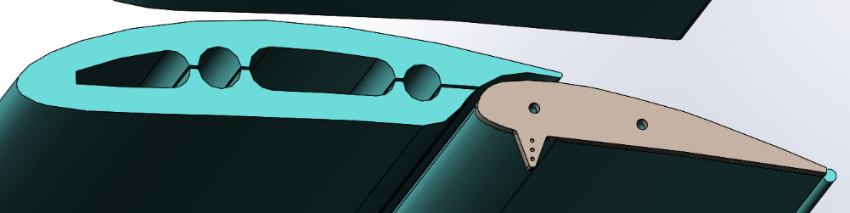
\includegraphics[width=\textwidth]{retracted-flap}
        \caption{Retracted}
        \label{fig:flaps:retracted}
    \end{subfigure}
    \hfill
    \begin{subfigure}[b]{0.49\columnwidth}
        \centering
        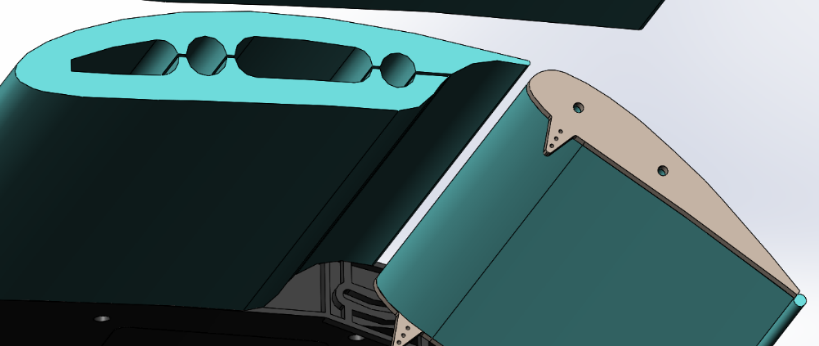
\includegraphics[width=\textwidth]{deployed-flap}
        \caption{Deployed}
        \label{fig:flaps:deployed}
    \end{subfigure}
    
    \caption{flap, with endplates for horn controls.}
    \label{fig:flaps}
\end{figure}

\subsection{Landing gear} \label{sec:design-process:design-revision:landing-gear}

Two main types of landing gear design were considered for this project: the tricycle and a tail wheel approach.
A tricycle consists of a single front wheel, and two rear wheels, as seen on most commercial aircraft; whereas a tail wheel design uses a single rear wheel with two front wheels.

\importtable{| >{\raggedright\arraybackslash}p{0.12\columnwidth} | >{\raggedright\arraybackslash}p{0.36\columnwidth} | >{\raggedright\arraybackslash}p{0.36\columnwidth} |}{
    \hline
    \textbf{Design} & \textbf{Advantages} & \textbf{Disadvantages} \\
    \hline
    Tricycle & Prevents nose tipping; improved stability; better manoeuvrability; better in crosswinds & Increased drag and weight; nose gears are prone to damage \\
    \hline
    Tail wheel & Lighter; easier to integrate with under rudder; more suitable for integration with nose design; propellors would have more ground clearance & Harder to attach front wheels; harder to manoeuvre \\
    \hline
}{tradeoffs involved in the gear layout used.}{gear-layout-tradeoffs}

When the landing gear was first being designed weight was the limiting factor, with the UAV close to the \kg{7} mass limit.
Because of this the decision was made to use a tail wheel approach as it is lighter than the tricycle approach.
The modularity and moving centre of gravity was a challenge unique challenge to this UAV, however, and the first step of the design was the calculation of the maximum loading conditions the landing gear would encounter \cite{goud-14}. 

\importimage{moment-calculations}{moment calculations.}{Moment calculations}{0.7}

The forwardmost centre of gravity (CG) meant $x=150\,\mathrm{mm}$ and $y=765\,\mathrm{mm}$, which led to a maximum static loading of \newtons{57.4} over the front wheels and \newtons{11.26} over the rear wheel.
The rearmost CG led to $x=200\,\mathrm{mm}$ and $y=815\,\mathrm{mm}$; the maximum static loadings for this condition are \newtons{55.13} and \newtons{13.53} over the front and rear wheels respectively.
Based on these calculations, a load of \newtons{57.4} and \newtons{13.53} were used in future calculations and analyses. 

That landing gear was designed to survive a ‘worst case scenario’.
If an issue were to occur during flight, the plane could still be controlled to a safe landing, if this was unable to happen, it was predicted that the UAV would not necessarily land on its landing gear.
Therefore, even during a failure, a vertical landing velocity of \mps{3} would be considered excessively large.
Using Newton's $2^\mathrm{nd}$ law, and an assumed impact time of 0.5 seconds, the maximum force of the UAV would be equal to \newtons{42}, meaning a total force of \newtons{110.67} on landing.
Since most UAVs land with their main wheels touching down first, the main landing gear must absorb the majority of the load: from previous calculations, the main gear should withstand \newtons{99.4}.  

\importimage{landing-gear-design-one}{landing gear design one.}{Landing gear design}{0.8}

A setting angle of \degr{5.8} was needed to meet takeoff requirements, as shown in Figure \ref{fig:landing-gear-design-one}.
To avoid hitting the rear propeller or the rudder, the rear wheel was designed to extrude from the bottom of the under-rudder.
The carbon fibre spar in the rudder would be strong enough to support the maximum \newtons{10} load it would encounter on landing. 

\importimage{landing-gear-attachment-locations}{potential landing gear attachment locations.}{Landing gear attachment locations}{0.7}

It immediately became clear that the main gear would have to be mounted to the main carbon fibre boom running the length of the fuselage.
Following advice from the project supervisor, however, it was decided that the main wheels should be located below the leading edge of the wing.
As Figure \ref{fig:landing-gear-attachment-locations} shows, mounting the main gear would not be possible in this location.
A solution involving having the main gear mounted further forward but curved backwards was investigated.  

Several iterations similar to the final design in Figure \ref{fig:main-gear-progression:final} were designed and tested using FEA.
The FEA was initially carried out on a single leg, with a loading of \newtons{50} applied to a fiberglass construction.
After the design of the leg was finalised a clamping system was devised to mount the main gear to the boom.
Further FEA showed that the clamping would be effective at attaching the fibreglass to the boom but would cause the boom to buckle on landing.
Figure \ref{fig:prepreg-cover-stress} shows how the addition of a prepreg cover around the boom significantly reduces the stress of the boom itself, roughly by a factor of 10. 

% \importimage{landing-gear-design}{main landing gear design.}{Landing gear design}{0.4}
\importimage{landing-gear-stress}{stress on landing gear.}{Landing gear stress}{0.5}
\importimage{prepreg-cover-stress}{effect of a prepreg cover on carbon fibre spar.}{Prepreg cover stress}{0.95}

At this point in the design process, the weight of the UAV was no longer an issue, and after a supervisor meeting in which the landing gear design was discussed it was decided that the landing gear should be steerable.
This would reduce the time taken time to retrieve the UAV upon landing as well as making takeoff easier.
The tail wheel setup is not optimal for a steerable configuration and so, as the fuselage and the weight of the aircraft had been reduced $-$ making weight less of a limiting factor $-$ the decision was made to redesign the landing gear in a tricycle configuration. 
FEA was carried out on the design and small changes were made until an optimal design was found.

\begin{figure}[H]
    \centering
    \begin{subfigure}[b]{0.33\columnwidth}
        \centering
        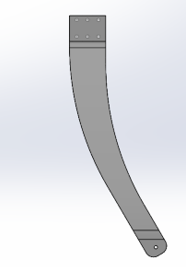
\includegraphics[width=\textwidth]{landing-gear-design}
        \caption{Initial}
        \label{fig:main-gear-progression:initial}
    \end{subfigure}
    \hfill
    \begin{subfigure}[b]{0.49\columnwidth}
        \centering
        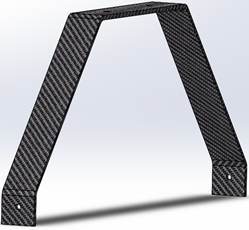
\includegraphics[width=\textwidth]{main-gear-design}
        \caption{Final}
        \label{fig:main-gear-progression:final}
    \end{subfigure}
    
    \caption{progression of the main gear design.}
    \label{fig:main-gear-progression}
\end{figure}


\subsection{Nose} \label{sec:design-process:revised-design:nose}

The nose was a key component in the project and needed to fulfil several criteria:

\begin{itemize}
    \item support a motor and propellor unit;
    \item provide access to the motor for removal;
    \item be removable from the rest of the fuselage whilst being strong enough to support the motor during flight;
    \item integrate the landing gear.
\end{itemize}

To fulfil all the above criteria, it was obvious from the start that the nose would have to be 3D printed, meaning there were no geometry restrictions placed upon the design. 
The initial design was simple, incorporating the ability to attach the motor via four internal screw holes.
The nose would be attached to the fuselage via a spar running through the nose and the front of the spar.
Although not optimal, at the time it was deemed acceptable to drill through the end of the carbon spar as it was away from the structural core of the fuselage.
The design also incorporated a slot for the battery to slide into to act as a ballast, as well as a slot for the ESC, which would maximise airflow to it for cooling purposes.

\begin{figure}[H]
    \centering
    \begin{subfigure}[b]{0.6\columnwidth}
        \centering
        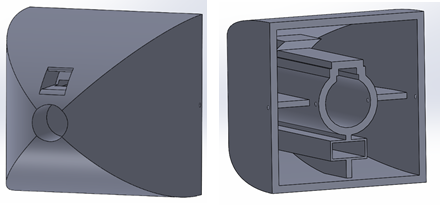
\includegraphics[width=\textwidth]{initial-nose-design}
        \caption{Initial}
        \label{fig:nose-design-progression:initial}
    \end{subfigure}
    
    \begin{subfigure}[b]{0.6\columnwidth}
        \centering
        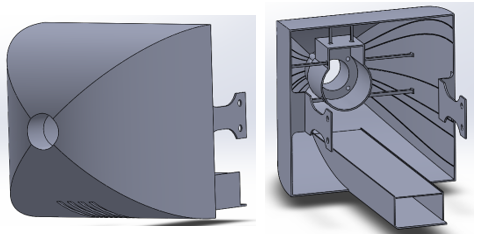
\includegraphics[width=\textwidth]{revised-nose-design}
        \caption{Revised}
        \label{fig:nose-design-progression:revised}
    \end{subfigure}

    \begin{subfigure}[b]{0.6\columnwidth}
        \centering
        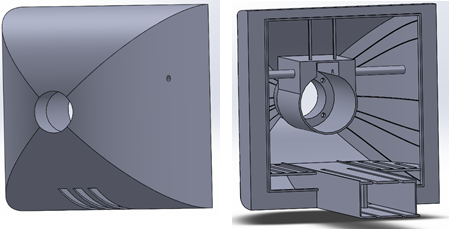
\includegraphics[width=\textwidth]{twice-revised-nose}
        \caption{Final}
        \label{fig:nose-design-progression:final}
    \end{subfigure}
    
    \caption{various stages of the design of the printed nose.}
    \label{fig:nose-design-progression}
\end{figure} 

% \importimage{initial-nose-design}{initial nose design.}{Initial nose design}{0.6}

Figure \ref{fig:nose-design-progression:revised} shows an updated version of the nose design.
Firstly, the outer body was lightweighted considerably from \mm{5} to \mm{1.5}, and supports were added.
The battery compartment became a tray, which will serves to make removal easier.
The tray had a section underneath in which the ESC was to be placed, with cooling vents in the front of the nose.
The nose was to be secured to the fuselage via two bolts along the width of the fuselage.
More light weighting was done to the motor support and rods used in place of the previous bulky design. 

% \importimage{revised-nose-design}{revised nose design.}{Revised nose design}{0.7}

After advice from the project supervisor, alterations were made to the revised design.
Most notably, a battery and ESC tray were added to the back of the nose, with vents in the front of the nose to allow cooling to the ESC.
The tray was supported by two vertical poles to support the weight of the battery. 

% \importimage{twice-revised-nose}{twice revised nose design.}{Twice revised nose design}{0.7}

The nose would now be secured by one bolt, through the carbon fibre spar, which would also act as a support for the motor mount.
After further deliberation with the project supervisor, however, it was decided that the loss in structural performance from drilling through the carbon fibre boom was not worth the reduction in workload, so a new way of attaching the nose to the fuselage was sought.  

The new multi-component nose design had two components.
The inner component would be secured to the fuselage at all times, and the front part would be removeable.
The inner part would be secured to the boom using a clamping mechanism, originally devised for the landing gear, via three M3 bolts located underneath the boom.
The outer part would then twist into the inner part and be locked in place using two M3 bolts. 

% \importimage{nose-inner-section}{inner section of the nose.}{Nose inner section}{0.7}

The inner part would had a \mm{1} wall thickness, supported by \mm{5} deep and \mm{3} wide support structures common on 3D printed UAV components as they are such a light way of increasing strength.
The clamping system was supported by a web-like structure.
The battery tray and ESC compartment were given a small redesign, with two larger vents channelling airflow to the ESC.
The steerable landing gear were also incorporated into the design, through the air vents. 

% \importimage{nose-outer-section}{outer section of the nose.}{Nose outer section}{0.7}

The outer section would be held in place via a twist and lock system.
To remove the front section, two screws would be removed from the side of the nose; the front would then twist anticlockwise and be removed.
Once removed, the electronics inside could be easily removed over the battery tray.
The motor could easily be removed via four screws located towards the front of the nose and replaced by a 3D printed part for aerodynamic purposes when the nose motor is not in use.
The motor mount area was also lightened, with similar structural supports on the \mm{1} outer wall. 

FEA was carried out on the outer section to ensure it was strong enough to support the fuselage.
Figure \ref{fig:outer-nose-fea} shows a \newtons{140} force applied to the locking tabs.
For SLS nylon the yield strength was set at 60 Mpa.
With the \newtons{140} load applied, however, the maximum stress reached was 5.582 MPa, resulting in a maximum displacement of \mm{0.1}. 

\begin{figure}[H]
    \centering
    \begin{subfigure}[b]{0.6\columnwidth}
        \centering
        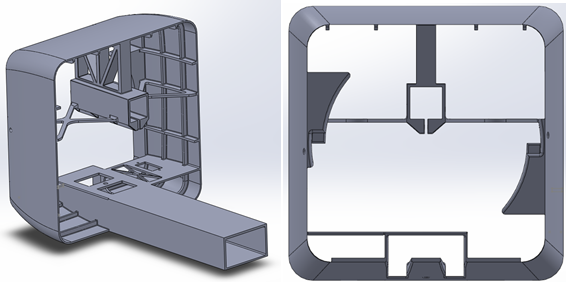
\includegraphics[width=\textwidth]{nose-inner-section}
        \caption{Inner section}
        \label{fig:nose-design:inner}
    \end{subfigure}
    
    \begin{subfigure}[b]{0.6\columnwidth}
        \centering
        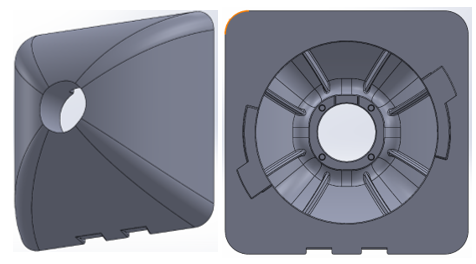
\includegraphics[width=\textwidth]{nose-outer-section}
        \caption{Outer section}
        \label{fig:nose-design:outer}
    \end{subfigure}

    \begin{subfigure}[b]{0.6\columnwidth}
        \centering
        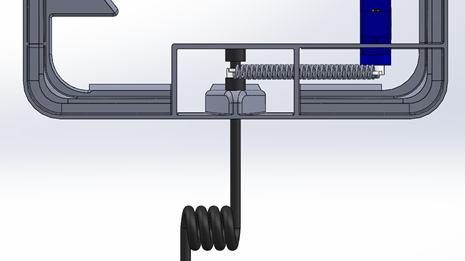
\includegraphics[width=\textwidth]{steerable-gear}
        \caption{Steerable gear attachment}
        \label{fig:nose-design:steerable-nose-gear}
    \end{subfigure}
    
    \caption{detailed models of the final nose design.}
    \label{fig:nose-design}
\end{figure} 

\importimage{outer-nose-fea}{FEA on the outer nose join.}{Nose join FEA}{0.7}

\subsection{Tail} \label{sec:design-process:revised-design:tail}

The tail is required to provide adequate stability to the aircraft in all stages of flight, as well as house the elevator and rudder control surfaces.
Design for the tail and stability systems was restarted following research and dialogue with the project supervisors after the wind tunnel test, which revealed the true scope of the design process required. 

Revision began with the tail surfaces themselves.
As the centre of gravity of the aircraft would not be in line with the centre of lift, the tailplane would need an angle of attack that would facilitate the aircraft's trim, and provide stability throughout flight, with minimal to no trim from the elevators at cruise speed.
The sizing of the tail surfaces and their angles were again determined using processes described by Sadraey \cite{sadraey-13}.
In particular an example of tail design was followed from \S 6.1 (and slightly modified) to obtain the tail dimensions and setting angle. 

The process began similarly to that of the wind tunnel model.
Revised volume coefficients were suggested as 0.8 for the horizontal tail, and 0.06 for the vertical tail \cite{towell-19}.
The tail planform area was determined as $0.16 \mathrm{m^2}$ for the horizontal tail, and $0.08 \mathrm{m^2}$ for the vertical tail.  % TODO: work out where these equations went (originally [1] and [2])

Next, the cruise lift coefficient was determined, using equation 6.27 from \cite{sadraey-13}, and was found to be 0.4671, based on a weight of \kg{7} (\newtons{68/67}), cruise speed of \mps{20}, and wing planform area of $0.6 \mathrm{m^2}$.
The wing/fuselage aerodynamic pitching moment coefficient then needed to be estimated.
Sadraey provided an equation for this, but at the suggestion of the project supervisor, equation E-40 $-$ which determined the change in wing pitching moment due to the fuselage $-$ from E. Torenbeek’s book \cite{torenbeek-76} was used instead.
This was determined to be $-0.0398$.
Based on a chart from 'Airfoil Tools' for the NACA6412 aerofoil, the wing 0 lift pitching moment coefficient was determined to be -0.137 \cite{airfoil-tools-19}.
This and the fuselage offset were then summed to give a value of the wing/fuselage pitch moment coefficient of $-0.1768.$ 

The next stage of the process required values for the centre of lift and mass locations in terms of percent of the MAC of the wing.
As these were unknown at this stage, they were estimated to be $h = 0.25$ (quarter chord) for the centre of lift (a reasonable assumption for most wings) and $h_0 = 0.5$ (half chord) for the centre of mass, which was a worst case value. 

Next, the required lift coefficient of the horizontal tailplane needed to be determined.
Essentially, the moment caused by the lift, thrust and weight, as well as the wing pitching moment, has to be counteracted by a moment provided by the tail.
It was decided that this should be negated at the cruise speed of the UAV, reducing the work required by the pilot for the majority of the flight.
The tail uses a symmetrical aerofoil, and as such provides no lift force at \degr{0} incidence, so requires a mounting angle to provide a balancing moment.
This has to take into account changes to flow incidence caused by the fuselage angle of attack at cruise to make the wing provide sufficient weight, balancing lift $-$ as well as flow downwash $-$ caused by the wing. 

To calculate the tail cruise lift coefficient, equation 6.29 from Sadraey \cite{sadraey-13} could be used; the project supervisor, however, suggested a method which rearranged a substituted force and moment balance of the aircraft in cruise, which resulted in an equation for the angle of attack of the fuselage relative to the wing zero lift line: 

\importequation{
    \alpha_{F_{0L}} = \frac{
        \frac{2mg}{V^2} + \frac{C_{m0}c}{l}
    }{
        \rho S C_{L\alpha} (1 + \frac{h-h_0}{l})
    }
}{tail-cruise-lift-coefficient}

At \mps{20}, the fuselage angle was determined to be 0.0944 radians (relative to wing zero lift).
The tail cruise lift coefficient could then be determined using a modified version of equation 6.29 from Sadraey \cite{sadraey-13} as $-0.0871$.
Using an equation for the lift coefficient $C_\mathrm{L} = C_{L\alpha}\alpha$, the required incidence of the tail could then be determined as \degr{-1.238}.  % TODO: add mathrm inside $
The fuselage angle of attack had been determined relative to the wing zero lift line previously.
The wing zero lift line was \degr{5.7}, and the wing was mounted at \degr{2}, giving the wing zero lift line as \degr{7.7} relative to the fuselage datum.
This gave the fuselage angle of attack in flight as \degr{-2.294}.  

The wing downwash calculation required the downwash at zero angle of attack, and the downwash curve slope.
These were both determined using equation E-52 in \cite{torenbeek-76}: calculating these values and substituting into the equation for downwash gave a value for the downwash caused by the wing, at the tail as \degr{1.924}.
Finally, the tail setting angle could be calculated, which resulted in a setting angle relative to the fuselage datum of \degr{2.979}. 

% \importimage{resulting-tail-design}{the resulting tail design.}{Resulting tail design}{0.4}
% \importimage{resulting-tail-design-side}{the resulting tail design, viewed from the side.}{Resulting tail design side}{0.4}

\begin{figure}[H]

    \centering
    \begin{subfigure}[b]{0.49\columnwidth}
        \centering
        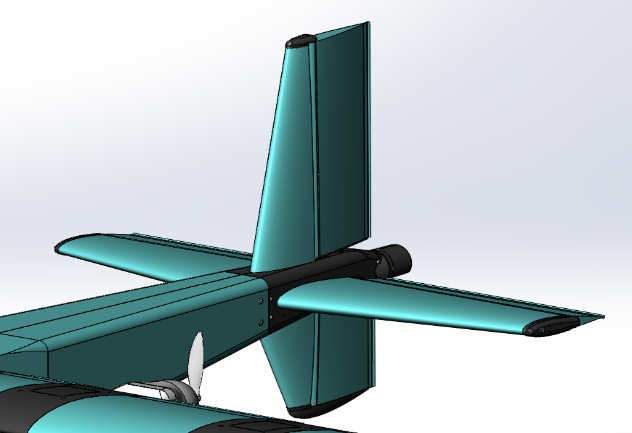
\includegraphics[width=\textwidth]{resulting-tail-design}
        \caption{}
        \label{fig:final-tail-design:angle}
    \end{subfigure}
    \hfill
    \begin{subfigure}[b]{0.49\columnwidth}
        \centering
        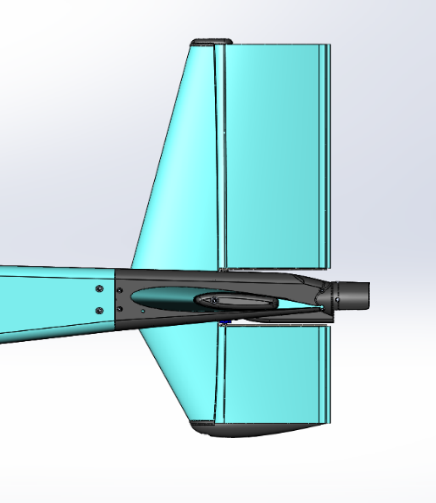
\includegraphics[width=\textwidth]{resulting-tail-design-side}
        \caption{}
        \label{fig:final-tail-design:side}
    \end{subfigure}
    
    \caption{resulting tail design.}
    \label{fig:final-tail-design}
\end{figure} 

One verification was to calculate the pitch stability derivative, using equation 6.67 in \cite{sadraey-13}, which resulted in $-0.6301$.
A negative value indicates that the pitch moment decreases with $\alpha$, which is desirable.
Following a process from \cite{de-kat-17} gave a stick fixed static margin of 0.1574, and a stick fixed manoeuvre margin of 0.2747, both of which are deemed to be acceptable values. 

Work on the yaw control requirements of the aircraft led to the decision to have an upper and lower vertical stabiliser, since extra rudder area was required, and to act as a bumper so that in the tail pusher propeller configuration $-$ where take off rotation or a hard landing might lead to tail propeller contacting the ground $-$ the propeller and therefore the aircraft would be protected.
Mounting a wheel on this bumper was considered when the UAV was planning use a tail wheel configuration, but when a nose wheel configuration was eventually settled upon, the bumper remained. 

The yaw stability of the aircraft was briefly checked following the addition of the extra rudder area, using equation  6.73 from Sadraeys book, the yaw stability derivative was calculated as 0.253, which was acceptable (it need only be positive, through the more positive the better).

Tail spars were resized using the same process as the wind tunnel model, as it had been decided to switch to pultruded carbon fibre rather than aluminium to save weight and move the centre of gravity forward.
The process does not account for the bonding of the extra foam material to the spars, so the estimated deflection would likely be pessimistic.  

Calculations from \cite{bresloff-18} were made to assess the potential effect of gusts and manoeuvres on tail loading through equations provided as the result of analytical processes in the lecture notes, which calculated the tail load in a symmetrical manoeuvre, and the additional load due to a gust encounter..
It was estimated that the maximum load likely to be seen in a gust encounter at the predicted flight altitude was approximately \newtons{39}.
The maximum expected load from a manoeuvre was approximately \newtons{14}, both within the $10g$ limit load for which the aircraft was designed. 

\subsection{Control surfaces} \label{sec:design-process:revised-design:control-surfaces}

The control surfaces were designed around their ability to meet several criteria that commercial aircraft must satisfy to be airworthy.
While the ELMO UAV is not required to meet the same stringent safety standards, many are there simply to ensure the aircraft flies properly, so it was prudent to meet them.
As such, the rudder was designed to maintain trim control in the unlikely event of a wing tip motor failing resulting in worst case asymmetric thrust.  

To begin, the rudder was parameterised in terms of the ratio of its chord to the root chord of the vertical stabiliser, its span, and its inside offset from the root of the stabiliser, allowing space for the servo.
Several useful parameters were derived from this including the MAC ratio, which was used on a plot from Sadraey \cite{sadraey-13} to find the angle of attack effectiveness $\tau$ of the rudder, which was used to calculate the rudder control derivative using equation 12.100 in \cite{sadraey-13}.
The rudder was modelled to be functioning at the predicted stall speed of the aircraft as it would be expected to maintain control at this speed.
A maximum deflection of \degr{30} was selected based on \cite{sadraey-13}, and then this and relevant values were substituted into equation 12.104a \cite{sadraey-13} to calculate the vertical stabiliser lift with a deflected rudder. 

The first version of this with only the upper vertical stabiliser yielded a lift of \newtons{5.08}.
This required comparing to the moment from the tip motor at full thrust, at stall speed.
The thrust of the motor changes with the inflow velocity.
Analysis of motor test data gave the thrust at predicted stall speed to be \newtons{8.73}.
The wing had a semi-span of \metres{1}, so this force is equal to the moment theoretically created in an asymmetric thrust scenario at this speed.
The tail arm was initially to be \metres{1}, but was reduced to \metres{0.9} for the purpose of moving the centre of mass forward, giving a tail moment of \Nm{4.57}, which is approximately half of that required by the asymmetric thrust scenario.
This design flaw, combined with the fact that the rear propeller in that configuration would be unprotected on rotation or a hard landing, led to the decision to add a lower vertical stabiliser, despite it being surplus to the required vertical stabiliser area. 

The upper stabiliser was extended very slightly, the same root and tip chords maintained for upper and lower stabilisers, and simply a span extended below the fuselage until it extended approximately an inch beyond the lowest reach of the rear propeller, visible in Figure \ref{fig:tail-assembly:horizontal-stabiliser}.  % TODO: check this reference 

The values of both spans were altered until the force created by the deflected rudder was sufficient to counteract the moment from the asymmetric thrust.
The increase of the span had the effect of increasing the effective aspect ratio of the vertical stabiliser, which increased the efficiency, and thus the 3D lift curve slope, so doubling the area was not required. 

The calculation was run with different speed values in Excel, to plot the rudder effectiveness and the motor thrust moment, over the expected speed range of the UAV (Figure \ref{fig:rudder-thrust-moment}).

\importimage{rudder-thrust-moment}{rudder against thrust moment at various speeds.}{Rudder against thrust moment}{0.95}

With this requirement satisfied, design of the rudder was concluded.
The lack of runway landing and already excessive rudder size lead to the decision to forgo other rudder validation tests. 

The next stage of the design was the elevators, which began with parameterised geometry of the elevator through a root chord ratio.
A value of a quarter chord was selected initially, and this proved to be more than sufficient for all subsequent analyses, and so remained.
The elevators took up all available trailing edge span of the horizontal stabiliser, leaving only room for the servo required to control it.  

The first attempt at the analysis of required deflections implemented a MATLAB code from \cite{sadraey-13} \S 12.8.2, in Excel, to plot out the elevator deflections for the most fore and aft centre of gravity, and over the predicted speed range of the UAV.
The output of this code appeared to not be able to capture the zero elevator deflection required at cruise speed (as the tail mounting angle has been designed around this).
The project supervisor provided another method to try before assuming that the tail mounting angle calculations were wrong.  

The process given started with a moment balance about the centre of gravity of the aircraft including lift, tail lift, wing pitch moment equated to the tail lift moment.
This could have values substituted in for lift, and be rearranged for the tail lift coefficient: 

\importequation{
    C_{L_h} = \frac{q S C_L (h-h_0) c + T z_T + q S C_{M_0}}{q S_h l}
}{cog-moment-balance}

Then performing analysis of forces in vertical equilibrium, rearranging and substituting for the tail lift coefficient above and rearranging for $\alpha$, yields the fuselage angle of attack at a given cruise condition: 

\importequation{
    \alpha = \frac{2 (mgl - Tz_T) V^{-2} - c C_{M_0}}{\rho S C_{L_\alpha}(l + (h - h_0)c)}
}{vertical-equilibrium}

With $\alpha$ found for a range of speeds, it could be used to find the tail lift coefficient for that particular speed, which is found by a rearranged version of the equation for tail lift coefficient, noting $\frac{S_h l}{Sc} = \overline{V}_h$, yielding: 

\importequation{
    C_{L_h} = \frac{C_{L_\alpha}\alpha(h-h_0) + \frac{Tz_T}{qSc} + C_{M_0}}{\overline{V}_h}
}{rearranged-tail-lift-coefficient}

With this, the elevator deflection can finally be calculated using:

\importequation{
    \delta = \frac{C_{L_h}}{C_{L_{\alpha_h}}} - \alpha (1 - \epsilon_\alpha) - \epsilon_0 - \frac{\alpha_h}{\tau_e}
}{elevator-deflection}

The process used above, along with the failed MATLAB code, repeated for a range of speeds yielded this plot (see legend for details):

\importimage{elevator-deflection}{elevator deflection plots for both processes.}{Elevator deflection plots}{0.95}

The second process captured the zero deflection required at cruise speed, and appeared to be correct, so design was concluded as satisfactory in this case.
Additionally, the deflections required from below the stall (and takeoff) speed are within the maximum deflections of the elevator selected.
The last test for the elevator was that it was satisfactory for aircraft rotation performance, which was based on a process from section 12.8.2 in \cite{sadraey-13}, and involved determining all forces and moments on the aircraft for the elevator to overcome on aircraft rotation.
To begin, the takeoff induced drag factor was determined using equation 5.22 in \cite{sadraey-13}, then this and other pre-determined values were used to determine the takeoff drag coefficient using equation 5.68 from \cite{sadraey-13}.
This was then used to determine the takeoff drag using the basic drag equation at a takeoff speed of \mps{13} and a value of \newtons{11.56} was calculated.  

Next the pitching moment of thw ing about the aircraft main gear was estimated as the wing zero lift pitch moment coefficient, and then a basic pitch moment equation to determine the moment on take-off as \Nm{-2.55}.
The aircraft's linear acceleration on rotation was then determined using equation 12.55 \cite{sadraey-13} with an estimated friction coefficient of grass from Table 9.7 \cite{sadraey-13}. 

Next, several geometric parameters of the aircraft were determined from the CAD model to be then substituted into equation 12.72 \cite{sadraey-13} to determine the lift required of the tail to achieve a set angular acceleration given the aircraft's mass moment inertia about the pitch axis.
This yielded a tail lift of \newtons{-3.17}, which gave a tail lift coefficient of $-0.192$.
Checking using the method defined previously to determine the elevator deflections at various speeds gave a required deflection of \degr{-7.59}, which is less than the maximum of \degr{-25}, so this is acceptable.
This concluded elevator design. 

Finally, the ailerons required sizing.
This was based around their ability to reach a required roll angle within a set time.
This requirement varies based on the aircraft type and flight phase, which was determined from table 12.12b \cite{sadraey-13} as a class II at phase C, at level 1, yielding the requirement that the aircraft reach a bank angle of \degr{30} within 1.8 seconds, with the additional requirement that this be in the configuration of the aircraft that would give the lowest roll rate with these ailerons (wing tip motors, giving a high mass moment of inertia about the roll axis).
The ailerons were parameterised by chord ratio (beginning with a value of 0.25, which proved satisfactory, so remained), and their inboard and outboard spans, however these were limited by the motor mount locations, so the main value to iterate upon was the chord ratio.  

A process from \S 12.8.1 \cite{sadraey-13} was used to determine aileron performance, beginning with the determination of the angle of attack effectiveness of the ailerons using the same method as previously.
This and several parameters were used in Equation 12.23 \cite{sadraey-13} to determine the aileron rolling moment coefficient derivative, yielding a value of \radsec{0.273}, which was then used to determine the aileron rolling moment coefficient at the maximum deflection of the aileron using Equation 12.13 \cite{sadraey-13}, which gave a value of 0.095. 

The ailerons need to be effective at an estimated approach velocity of 1.1 times the stall speed.
The aileron lift was determined at this speed using Equation 12.11 \cite{sadraey-13}, which resulted as \newtons{10.04}.
This was then used to determine the steady state roll rate using Equation 12.37 \cite{sadraey-13}, which gave a value of \radsec{7.14}.
This steady state roll rate was then used to determine the bank angle at which the steady state roll rate would be achieved, using Equation 12.43 \cite{sadraey-13}, which gave a value of \degr{74.57}.
The rate of roll rate could then be calculated using the steady state roll rate and time to reach it, using Equation 12.49 \cite{sadraey-13}, which gave a value of \radsecsec{0.342}.
Finally, the \degr{30}  bank angle requirement and rate of roll rate were used to determine the time to reach the bank angle of \degr{30} using Equation 12.47 \cite{sadraey-13}, which resulted in 1.75 seconds, less than the maximum 1.8 seconds; so the aircraft satisfied roll control requirements.
The time reduced to 1.17 seconds for the same process repeated at cruise speed. 

To conclude control surface mathematical design, it was checked using XFOIL that the servos chosen would be able to cope with the hinge moments.
For aesthetics it was chosen to have the servo axis in line with the control surface axis.
This removes the need for horn controls.
A code was used that yielded a hinge moment coefficient, which was then multiplied by relevant values to obtain the hinge moment.
As the servo and control surface axes were in line, if this value was greater than the stall torque of the servo, the servo was deemed inappropriate.
The SG90S had been selected, and was appropriate for all control surfaces, apart from the upper rudder, which was later changed to a HITEC HS 85 MG servo, which had sufficient stall torque. 

% \importimage{elevator}{a single elevator.}{Elevator}{0.4}
% \importimage{transparent-stabiliser}{a transparent view of the assembly of one horizontal stabiliser and elevator.}{Horizontal stabiliser}{0.4}

\begin{figure}[H]

    \centering
    \begin{subfigure}[b]{0.49\columnwidth}
        \centering
        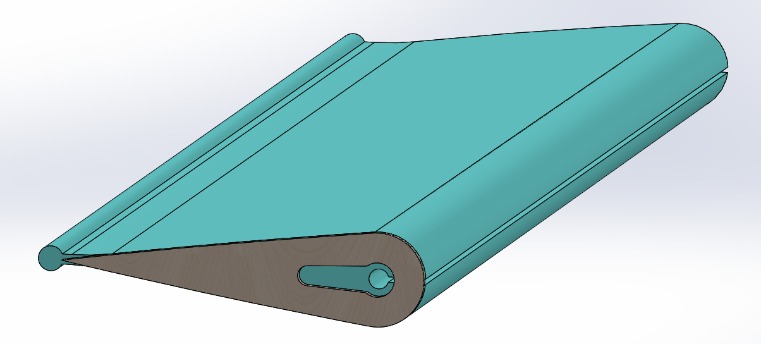
\includegraphics[width=\textwidth]{elevator}
        \caption{Elevator}
        \label{fig:tail-assembly:elevator}
    \end{subfigure}
    \hfill
    \begin{subfigure}[b]{0.49\columnwidth}
        \centering
        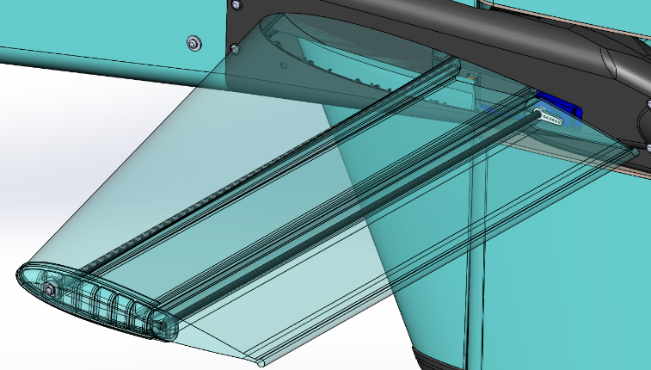
\includegraphics[width=\textwidth]{transparent-stabiliser}
        \caption{Horizontal stabiliser}
        \label{fig:tail-assembly:horizontal-stabiliser}
    \end{subfigure}
    
    \caption{components of the horizontal component of the tail section.}
    \label{fig:tail-assembly}
\end{figure} 

The rudder basic shape was cut out from a duplicate of the vertical stabiliser model.
The space for the servo was cut out from the root, then additional cut-outs made for the stiffening spar near the leading edge, and foam cutter wire paths.
Next a thin second body was extruded from the root to define a laser cut profile that would allow for the servo arm to have a place to nest into, allowing for control of the rudder.
Lastly a small circular profile (designed to be cut off manually at a later stage) was extruded on the trailing edge so that the foam cutter would not damage the trailing edge since it was so thin.
The secondary rudder and elevators were defined identically. 

The ailerons were generated from a sketch of the aerofoil profile which was defined from the wing profile sketch, then one aileron extruded in a long profile.
Planes were then defined in the model that referenced the motor mount surfaces in contact with the aileron root and tip surfaces.
Material outside these two planes was then removed to define one aileron, which was then mirrored about the centre plane, defining both ailerons in a way that would instantly react to changes in motor mount location and spans between them.
Next, a small amount was cut off the roots of the ailerons and replaced with a small laser cut profile extruded outwards, similarly to the tail control surfaces that allowed for the inline servo arm to control the aileron.
Finally, holes were added for a stiffening spar, and wire paths added for the foam cutter. 

\subsection{Electronics} \label{sec:design-process:revised-design:electronics}

With the choice of flight controller finalised, the only other critical component of the electronics was the receiver.
Once the model of the receiver was also known, the type and quantity of wires that would be needed to distribute power and control signals to the rest of the aircraft could be determined.

\subsubsection{Receiver} \label{sec:design-process:revised-design:electronics:receiver}

The model of receiver that could be used was constrained primarily by the model of transmitter to which it would be bound.
While a Futaba transmitter was originally to be loaned from the university, scheduling constraints resulted in its unavailability for the duration of the project.
As an alternative, a FrSky Taranis X9D transmitter was purchased upon recommendation of its being a good tradeoff between price and flexibility.
The model is widely used and compatible with a wide range of receivers, uses a standard communication protocol, and also runs a configurable operating system, OpenTx, which enables it to be programmed in Lua.
As well as the standard joysticks, the handset has triggers and switches which can be mapped to the flaps and autopilot channels. 

One further factor constrained the selection of receiver: the signal output protocol needed to be SBUS to be compatible with the Matek flight controller, and have at least eight output channels.
Other factors, while less important, included the power usage, cost, and size of the receiver.
The receiver was intended to fit onto an electronics tray along with the flight controller, and would be powered by the same battery as the flight controller, microcontroller, and servos.
A receiver, the FrSky X8R (Figure \ref{fig:flight-controller-receiver}), was found, operating on 100 mA at \volts{5} (the standardised output voltage of the flight controller), and weighing less than 20 g.
Its profile is also similar to that of the flight controller, meaning that it would not be the limiting factor in the size and shape of the electronics tray when the fuselage was designed. 

\importimage{flight-controller-receiver}{receiver undergoing the binding procedure.}{Receiver binding}{0.5}

When bound to a Taranis X9D, the X8R is capable of receiving sixteen independent channels via FrSky's radio transfer protocol ACCESS (a newer and more robust version of ACCST).
This would be more than sufficient for the eight channels required as a baseline for the project, and would also leave room for the expansion of the project with additional features, as mentioned previously, with the eight leftover channels.
The operating range of 1.5 km would also be more than sufficient for the project. 

As well as being compatible with the Taranis transmitter and capable of outputting to SBUS, the X8R had a number of serial ports (standard PWM outputs) which could be used for testing and validating its functionality without having to pass the signals through the flight controller first.
It was thought that this could be useful in the later stages of the project while troubleshooting any issues, being able to remove the flight controller from the loop and isolate the receiver to check that it was communicating properly with the transmitter.

\subsubsection{Servos} \label{sec:design-process:revised-design:electronics:servos}

All moveable surfaces on the aircraft were to be actuated by servos.
These are split into four groups: ailerons, elevators, rudder, and flaps.
The first three are the control surfaces by which the aircraft is controlled, and would need to be sized for a fairly limited selection of manoeuvres.
It was not expected that the aircraft would be performing any tight turns, but the load that would be transferred through the aileron servos could depend greatly on the configuration of the PUCs.
With the units located at the end of the wings, the greatly increased moment of inertia of the aircraft would mean that actuating the ailerons would not produce nearly as much inertial relief as when the motors and batteries were located on the centreline.
As such, the servos could be expected to see a fairly variable range of loads.
In addition, the loads experienced by the rudder servos was found to be far in excess of the loads experienced by all other servos when the possibility of an asymmetric motor failure at the wingtips was considered.
It was decided that these servos would need to be of a different type to those elsewhere in the aircraft. 

In all, fourteen servos were required to control the aircraft, including the two servos of different specification for the rudder.
The exact configuration of these servos, as well as the signals passed to each of them, is shown below. 

\importimage{signal-splitters}{control signal splitter schematic.}{Signal splitter schematic}{0.9}

Note that each flap is supported by two servos of opposing deflection directions.
While the flaps increase the lift of the aircraft quite dramatically, and thereby exert a large moment onto their supporting servos, the distribution of this load across four flap segments and eight servos meant that the smaller servo size was capable of holding the flaps in place during takeoff and landing. 

One potential issue with the servos selected was the degradation of the plastic-toothed gears they use.
Information from peers suggested that sufficient use would wear the gears down and reduce their effective strength, causing the gears to slide at a smaller load than suggested by the servos' data sheets.
An experiment was devised to repetitively test a servo under load (actuating it far more times than would ever be expected of a servo in a flight model) to see whether its strength afterwards was the same as upon its delivery; but this experiment was never carried out due to the COVID-19 pandemic.
In the event that it had been found to significantly impact the strength of the servos, metal-toothed servos could have been purchased at a slightly higher cost. 

\subsubsection{Avionics battery} \label{sec:design-process:revised-design:electronics:avionics-battery}

The entirety of the electronics subsystem was to be powered by a single battery, referred to as the avionics battery.
This would be connected to the flight controller, powering it directly, and indirectly powering the receiver, microcontroller, and servos.
While throttle signals would be supplied to the motors from the flight controller directly, the bulk of their power would come from the ESCs, which are in turn powered by the battery local to the corresponding PUC. 

In order to size the battery used for the avionics, the approximate power draw of each of the electrical components needed to be determined.
Research was conducted, considering the following items drawing power during a typical 10-minute flight: 

\begin{itemize}
    \item Servos
        \begin{itemize}
            \item Draw 10 mA while idle, 100 to 250 mA while moving, and have a stall current of 360 mA 
            \item The stall torque of the servos being used is 1.7 kg.cm, meaning that for a \cm{4} control surface, a load of roughly \kg{0.5} would need to be applied to cause a stall.
                Considering that there are nine control surfaces and that the total lift generated by the aircraft is around \kg{7}, it could reasonably be assumed that the likelihood of any individual control surface experiencing a load of \kg{0.5} is extremely small; certainly small enough that it would occur only momentarily and did not need to be factored into the draw calculations 
            \item 8 servos were used for the flaps and so would only move for a few seconds per flight 
            \item One servo was connected to the nose gear, which would likely only be moving periodically within two 30-second windows at the start and end of each flight 
            \item 5 servos were connected to the control surfaces.
                It was assumed that control surfaces would only move for around \pc{50} of the flight duration.
                To build in a bit of redundancy and account for the movement of the flap and gear servos, it was assumed that the power drain from servos would be equivalent to five servos moving constantly 
            \item This then equated to \amps{1} drawn by servos 
        \end{itemize}
    \item Receiver: listed as drawing a continuous 100 mA 
    \item Flight controller: listed as drawing a continuous 500 mA, a conservative estimate 
    \item The exact current draw of a microcontroller was difficult to determine as it depends primarily on how much the processor is being used.
        Even conservative estimates resulted in around 20 mA of draw, so that was neglected in this calculation as it is so much smaller than the other components 
\end{itemize}

An additional constraint placed on the battery was the required voltage of between 9 and 30 volts.
As the battery was required to be a LiPo battery, this limited the selection to those with between 3 and 6 cells. 

Assuming a total of 1600 mA drawn while in flight (a conservative estimate which also accounted for the small amount of additional power used for one-off events during takeoff and landing), and the voltage requirements, a few batteries were found which could power the avionics.
Several higher-capacity batteries were heavier and more expensive and, while they would enable multiple flights on one battery, switching out multiple lower-capacity batteries which were both lighter and cheaper was found to be more cost- and mass-effective, and also in keeping with the modular nature of the project. 

The battery settled on was therefore a 450 mA, \volts{11.1}, and 65 to 130 C discharge, which would provide for at least 15 minutes of flight on a conservative estimate of the power draw.
Its low cost meant that multiple could be bought and swapped out between flights, while used batteries are recharged.

\subsubsection{Foam model} \label{sec:design-process:revised-design:electronics:foam-model}

\importimage{bixler}{image of the Bixler 3 RC plane.}{Bixler model}{0.5}

Before the electronics were to be flown on the UAV they needed to be tested.
There was thorough testing of the electronics out of the aircraft first, but in order to be deemed flight worthy it needed to be tested in the air in a sacrificial flight vehicle.

The foam model selection was based on the constraints of the fuselage size required to fit all of the electronics inside, keeping the cost as low as possible, and having an aircraft that could be flown by the members of the project, with little to no flying experience.
The fuselage needed to be able to fit all of the necessity electronics: battery, ESC (which, in this case, was not stored in the PUC), receiver, Arduino, Matek, and GPS.

The optimal model was therefore a beginners' plane that had excess fuselage space, and so the Bixler 3 was chosen for its large internal cavities including an empty nose, giving ample room for the necessary components.
Furthermore, the plane is designed for beginners and so has a large surface area wing for low speed flying, high mounted wings for stability, a rear-facing motor and propeller above the fuselage to remove them from harm's way in the event of a crash, and a strengthened fuselage belly to act as a skid if the landing gear comes off in a particularly heavy landing.
All of this made it ideal for this use case.

\end{document}
